% !TEX program = xelatex
\PassOptionsToPackage{quiet}{xeCJK}
\PassOptionsToPackage{no-math}{fontspec}
\documentclass[11pt,oneside]{book}
\usepackage{geometry,enumitem}
\geometry{margin=1in}

\usepackage[hidelinks,colorlinks=true,linkcolor=teal,citecolor=violet,urlcolor=purple]{hyperref}

\usepackage{amsmath,amssymb,amsthm,mathrsfs}
\usepackage[lite]{mtpro2}
\usepackage[e]{esvect}
\usepackage{physics2,fixdif,derivative,cancel}
\usephysicsmodule{ab,ab.legacy,braket,nabla.legacy}
\theoremstyle{definition}
\newtheorem{problem}{Problem}[section]
\newtheorem{theorem}{Theorem}[section]
\def\theproblem{\arabic{problem}}
\newtheorem*{example}{Example}
\newtheorem*{solution}{Solution}
\numberwithin{equation}{section}

\usepackage{graphics,graphicx,pdfpages,paracol}
\graphicspath{{./figures/}}

\usepackage{fontspec,xeCJK}
\setmainfont{Libertinus Serif}
\setsansfont{Libertinus Sans}
\setCJKfamilyfont{cshk}{Chiron Sung HK}[BoldFont=Chiron Sung HK Bold]

\usepackage{indentfirst}
\setlength{\parindent}{2ex}

\usepackage[labelsep=period,labelfont={bf,sf},font=small]{caption}
\def\figref#1{\textsf{\textbf{Figure~\ref{#1}}}}

\usepackage{booktabs,tabularx}

\usepackage{tocloft}
\setlength{\cftbeforetoctitleskip}{-3ex}
\setlength{\cftaftertoctitleskip}{3ex}
\usepackage{titlesec}
\titleformat{\chapter}[hang]{\huge\bfseries\sffamily}
{\parbox{25mm}
    {\centering\HUGE\normalfont\bfseries\textcolor{gray}{\thechapter}\\[4mm]\normalsize\bfseries\textcolor{gray}{\bfseries\sffamily\textsc{Chapter}}}%
    \tikz[baseline]\draw[line width=3pt,dotted,dash pattern=on 0pt off 8pt, gray!50](0,-.9)--(0,1.5);
}{2ex}{}
\titlespacing{\chapter}{0ex}{0ex}{8ex}
\usepackage{pgfornament-han}

\usepackage{tikz}
\usetikzlibrary{arrows,tikzmark,patterns,calc}
\tikzset{>=stealth',
every picture/.append style={
    line join=round,
    line cap=round,
    thick
  }}

\makeatletter
\def\HUGE{\@setfontsize\Huge{50}{50}}
\renewcommand*\maketitle
{
\begin{titlepage}
    \newgeometry{margin = 0 in}
    \parindent=0pt
    \vspace*{8ex}
    
    \centering
    \ifcsname @title\endcsname
    \rule{.75\linewidth}{2pt}
    \HUGE\sffamily\bfseries\@title\\
    \vskip-1ex
    \rule{.75\linewidth}{2pt}
    \fi
    \vskip2ex
    \ifcsname @author\endcsname\huge\@author\fi
    \vskip2ex
    \ifcsname @date\endcsname\Large\@date\fi
    
    \vfill
    
    \tikz
    {
    \foreach \a in {1,2,...,17}
    \node [teal,xshift=\a*36,inner sep=0pt,] at (0,0) {\pgfornamenthan[scale=.2]{47}};
    }
    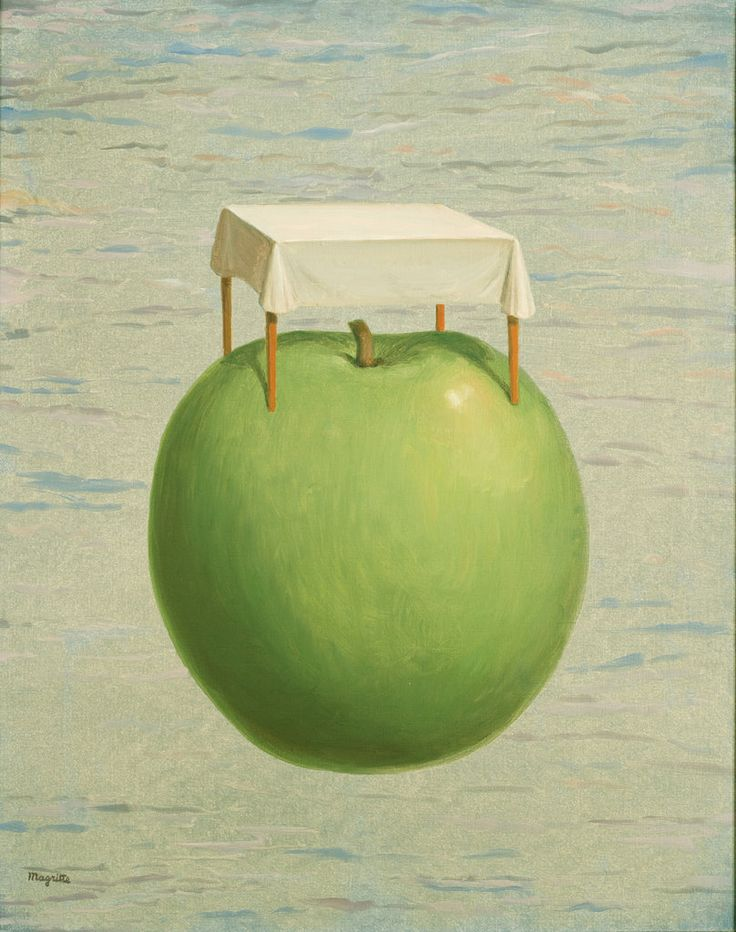
\includegraphics[trim={0 \dimeval{.5\paperheight} 0 0},clip,width=\paperwidth]{Beautiful realities, 1962;.jpeg}
    \restoregeometry
\end{titlepage}
}

\AtBeginDocument{
    \everymath{\displaystyle}
    \setlength{\abovedisplayskip}{3pt}
    \setlength{\belowdisplayskip}{3pt}
    \setcounter{tocdepth}{1}
}
\usepackage[toc]{multitoc}

\title{\textsc{General Relativity}}
\author{Robert M. Wald}
\date{The University of Chicago Press}

\begin{document}
\maketitle

\frontmatter\tableofcontents
\input{cha/copyright}

\chapter*{Preface}
\addcontentsline{toc}{chapter}{Preface}
This book is intended to provide a thorough introduction to the theory of general relativity. It is intended to serve as both a text for graduate students and a reference book for researchers. These two goals are somewhat contradictory, and to the extent that they are, part I of the book emphasizes the first goal. It treats the topics usually covered in introductory relativity courses: basic differential geometry, Einstein's equation, gravitational radiation, the standard cosmological models, and the Schwarzschild solution. More emphasis is placed on the second goal in part II of the book, which treats a wide variety of advanced topics. However, even here I have attempted to explain all the basic ideas at an introductory level.

If I were teaching a one term introductory course on general relativity, I would cover most of the material of part I together with much of appendices B and C. For a full year course, I then would choose several chapters from part II as the basis for the material covered in the second term. For example, chapters 8 and 9 and parts of chapter 12 could comprise a one term course on global methods. Chapter 7, supplemented by current literature, could serve as the basis for a course on methods for obtaining solutions. Chapter 10 and appendix E, supplemented by further reading, could be used for a course on the dynamics of general relativity. Chapter 12 (supplemented by background material from chapters 8, 9, and 11) and chapter 14 could comprise a course on the classical and quantum properties of black holes. It should be noted that the chapters in part II of the book are largely independent of each other and, for the most part, can be read out of sequence with the following major exceptions: prior reading of chapter 8 is essential for chapter 9, and chapter 8 together with parts of chapters 9 and 11 are essential for the first two sections of chapter 12.

One of the most difficult issues which arises during the writing of a book on general relativity is where in the book to present the rather substantial amount of mathematical material that is needed. Much of this material (e.g., tensor calculus and curvature) is required even for the formulation of general relativity. Some material (e.g., Lie derivatives and Killing fields) could be avoided initially but soon becomes necessary to make the discussion clearer and to simplify computations. Finally, some of the mathematical material (e.g., many of the theorems on topological spaces) is not really needed until part II of the book. If all this material were presented at the beginning of the book, it would comprise a truly formidable obstacle to learning general relativity. On the other hand, if the mathematical results were introduced only ``as needed'' in the later chapters, the mathematical discussion would become greatly fragmented and these fragments would interrupt the discussion of physical issues. The best solution I could find to this problem was to put all the mathematical material essential for the formulation of general relativity into chapters 2 and 3, and then to put the remaining mathematical topics into appendices A, B, and C. In this way, the reader can get to chapter 4 without unnecessary detours, but the discussion of all the mathematical topics remains intact and can be referenced as needed in the text. Thus, it should be emphasized that \emph{appendices A, B, and C are an essential part of this book}. The results derived in appendices B and C are used in many places throughout the book, and the definitions and results on topological spaces which are compiled in appendix A are referred to frequently in chapters 8 and 9.

One other somewhat unusual organizational feature of the book is that the Lagrangian and Hamiltonian formulations of general relativity also have been put in an appendix. Often, the Hamiltonian formulation is presented in conjunction with the initial value formulation of general relativity, but since the statements and proofs of the initial value results do not rely upon the Hamiltonian formulation, I found it logically clearer to discuss them independently. This left the Lagrangian and Hamiltonian formulations as topics which are unlinked to the material in the other chapters, too short to comprise a whole chapter on their own, and too important to omit. Thus, they ended up being treated in appendix E.

Problems are given at the end of each chapter in text. There is significant variation in the amount of thought and computation required to solve the problems, but there are very few trivial, ``mechanical'' exercises and none which are, in my opinion, inordinately difficult (i.e., I think I can solve them). Part of my purpose in giving some of the problems (particularly in the second half of the book) was to introduce important side points for which I did not want to make a detour in the text. Hence, even the reader who is determined not to do any exercises may still wish to read the problems.

I have benefited from numerous interactions with many colleagues while planning and writing this book. The influence of Robert Geroch should be apparent to readers familiar with his viewpoints on general relativity. Some of the arguments used in chapter 3 are adopted directly from the notes from a course we taught jointly in 1975. I particularly wish to thank colleagues who took the time and trouble to read parts (and, in a few cases, all) of the book and send me their suggestions for improvements. These include Abhay Ashtekar, Arvind Borde, S. Chandrasekhar, David Garfinkle, John Friedman, Robert Geroch, James Hartle, James Isenberg, Bernard Kay, Karel Kuchai, Liang Can-bin, Roger Penrose, Michael Turner, and William Unruh. Additional thanks are due David Garfinkle for checking most of the equations.

I wish to thank Susan Lancaster and Roxy Boersma for typing drafts of the manuscript and Fred Flowers for typing the final product on a word processor. Support by NSF grant PHY 80 26043 to the University of Chicago during the writing of this book is gratefully acknowledged. Finally, I wish to thank my wife, Veronica, for the considerable amount of patience displayed during the three years it took me to write this book.
\chapter*{Notation and Conventions}
\addcontentsline{toc}{chapter}{Notation and Conventions}
In this book we shall follow the sign conventions of Misner, Thorne, and Wheeler (1973). In particular, we use metric signature $-\ +\ +\ +$, we define the Riemann tensor by \eqref{3.2.3}, and we define the Ricci tensor by \eqref{3.2.25}. However, we shall make one important exception to these conventions. We choose to use the metric signature $-\ +\ +\ +$ because it is generally much more convenient than the alternative choice $+\ -\ -\ -$ in that it induces a positive definite (rather than negative definite) metric on spacelike hypersurfaces. Unfortunately, for the reasons explained in chapter 13, it is much more convenient to use the metric signature $+\ -\ -\ -$ for the treatment of spinors. Furthermore, the standard references on spinors all use this signature. \emph{Hence, in chapter 13-and only in chapter 13—we will change our metric signature convention to $+\ -\ -\ -$}. The confusion which might result from this should be minimized by the fact that the equations of chapter 13 are written in spinor notation, so the reader need only remember to change the sign of the metric when transcribing equations from spinor notation to tensor notation for use elsewhere in the book. With regard to these changes of sign, it is useful to note that the derivative operator, $\nabla_a$, associated with the metric is unaffected by a sign change of the metric. Hence, the Riemann tensor with index structure $R_{abc}^d$ also is unaffected, since it is defined purely in terms of $\nabla_a$. (However, it should be noted that some authors define the Riemann tensor with sign opposite that of \eqref{3.2.3}; see Misner, Thorne, and Wheeler (1973) for a table of sign conventions.) Similarly, it is conventional to take the stress-energy tensor $T_{ab}$ and Maxwell field tensor Fab to be unaffected by a change of metric signature. However, each raising or lowering of an index on $R_{abc}^d$, $T_{ab}$, $F_{ab}$, and any other tensor results in a change of sign.

Throughout most of this book, we shall use ``geometrized units'', where the gravitational constant $G$ and the speed of light $c$ are set equal to $1$. However, for the convenience of the reader we have restored the $G$'s and $c$'s in section 5.4 and in many of the formulas elsewhere in the book where observational predictions are made. A conversion table from ``geometrized'' to ``nongeometrized'' units is given in appendix F.

Our notation differs from standard conventions in one important respect. Most relativity texts use an index notation for components of tensors. Usually, greek indices are used to denote space or time components of a tensor, while latin indices are used to denote purely spatial components, although in some references (e.g., Landau and Lifshitz 1962) these conventions are reversed. This index notation provides an extremely efficient scheme for denoting tensor operations such as contraction, covariant differentiation, and the taking of outer products. However, this standard notational convention suffers from the serious drawback that it is impossible to distinguish a relation between tensors from a relation which holds only for tensor components with respect to a specially chosen basis. We shall overcome this difficulty by employing an abstract index notation discussed by Penrose (1968) and Penrose and Rindler (1984) and used extensively by Geroch. In our notation, latin indices on a tensor do not represent components but are part of the notation for the tensor itself, much like the arrow used to denote a vector in ordinary three-dimensional space. Thus, in this book any equation involving tensors which employs latin indices represents a relation between tensors; the taking of basis components need not even be contemplated. The complete rules for interpreting the notation are given in section 2.4. On the other hand, greek indices on a tensor represent components, as in the usual convention. Any equation employing greek indices is a relation between tensor components and, usually, holds only with respect to a specially chosen basis. Unfortunately, in our notation we cannot denote purely spatial tensor components without introducing yet another alphabet. However, only rarely in this book do equations arise which hold only for spatial components, and in such cases we simply shall state explicitly for which components a given equation applies.

For the benefit of the reader who is not well versed in mathematical notation, we list below the definitions of some of the standard mathematical symbols used frequently in the text

\begin{table}[!ht]
    \centering
\begin{tabularx}{\textwidth}{c X}
    \toprule
    $\cup$ & $A\cup B$ denotes the union of sets $A$ and $B$\\
    $\cap$ & $A\cap B$ denotes the intersection of sets $A$ and $B$\\
    $\subset$ & $A\subset B$ denotes that $A$ is a subset of $B$\\
    $-$ & $B-A$ denotes the complement in $B$ of the set $A$\\
    $\in$ & $p\in A$ denotes that $p$ is an element of $A$\\
    $\{|\}$ & $\{p\in A|Q\}$ denotes that set consisting of those elements $p$ of the set $A$ which satisfy condition $Q$\\
    $\times$ & Cartesian product; $A\times B$ is the set $\{(a,b)|a\in A \text{and} b\in B\}$\\
    $\varnothing$ & the empty set\\
    $\mathbb{R}$ & the set of real numbers\\
    $\mathbb{R}^n$ & the set of $n$-tuples of real numbers\\
    $\mathbb{C}$ & the set of complex numbers\\
    $\mathbb{C}^n$ & the set of $n$-tuples of complex numbers\\
    $:\ \to$ & $f:A\to B$ denotes that $f$ is a map from the set $A$ to the set $B$\\
    $\circ$ & $f\circ g$ denotes the composition of maps $g:A\to B$ and $f:B\to C$, i.e., for $p\in A$ we have $(f\circ g)(p)=f[g(p)]$.\\
    $[\ ]$ & f$[A]$ denotes the image of the set $A$ under the map $f$, i.e., the set $\{f(x)|x\in A\}$.\\
    $C^n$ & the set of $n$-times continuously differentiable functions\\
    $C^\infty$ & the set of infinitely continuously differentiable (i.e., smooth functions)\\
    \bottomrule
\end{tabularx}
\end{table}

In addition, a number of symbols defined in the book appear frequently and are not always redefined each time they are used. Hence, for the convenience of the reader we list these symbols below, together with the section of the book where they are defined

\begin{table}[!ht]
    \centering
\begin{tabularx}{\textwidth}{c X}
    \toprule
    $\overline{S}$ & the closure of the set $S$ (appendix A)\\
    $\text{int}(S)$ & interior of the set $S$ (appendix A)\\
    $\dot{S}$ & boundary of the set $S$ (appendix A)\\
    $\mathscr{L}_v$ & Lie derivative with respect to the vector field $v^a$ (appendix C)\\
    $\mathscr{F}$ & the set of smooth functions from a manifold $M$ into $\mathbb{R}$ (section 2.2)\\
    $V_p$ & tangent space at point $p$ of a manifold\\
    $V_p^*$ & dual space to $V_p$ (section 2.3)\\
    $I^+(S)$ & chronological future of the set $S$ (section 8.1)\\
    $J^+(S)$ & causal future of the set $S$ (section 8.1)\\
    $D^+(S)$ & future domain of dependence of the closed, achronal set $S$ (section 8.3)\\
    $H^+(S)$ & future Cauchy horizon of the closed, achronal set $S$ (section 8.3)\\
    $\mathscr{J}^+$ & future null infinity (section 11.1)\\
    $i^0$ & spatial infinity (section 11.1)\\
\bottomrule
\end{tabularx}
\end{table}

The symbols $I^-(S),\ J^-(S),\ D^-(S),\ H^-(S)$, and $\mathscr{J}^-$ are defined as above with ``past'' replacing ``future''. $D(S)$ denotes $D^+(S)\cup D^-(S)$, and $H(S)$ denotes $H^+(S)\cup H^-(S)$. Finally, round and square brackets around tensor indices denote, respectively, symmetrization and antisymmertrization, as defined by \eqref{2.4.3} and \eqref{2.4.4}.
\mainmatter
\chapter{Introduction}
\section{Introduction}
General relativity is the theory of space, time, and gravitation formulated by Einstein in 1915. It is often regarded as a very abstruse and difficult theory, partly because the new viewpoint it introduced on the nature of space and time takes some effort to get used to since it goes against some deeply ingrained, intuitive notions, and partly because the mathematics required for a precise formulation of the ideas and equations of general relativity (namely, differential geometry) is not familiar to most physicists. Although it has been universally acknowledged as being a beautiful theory, the potential relevance of general relativity to the rest of physics has not been universally acknowledged and, indeed, probably for this reason, the subject has lain nearly dormant during much of its history.

Strong interest in general relativity began to be revived starting in the late 1950s, particularly by the Princeton group led by John Wheeler and the London group led by Herman Bondi. Although it is difficult to determine the reasons for trends in physics, two developments-relating general relativity to other areas of physics and astronomy-have contributed greatly to the sustained interest in general relativity which has continued since then. The first is the astronomical discovery of highly energetic, compact objects-in particular, quasars and compact X-ray sources. It is likely that gravitational collapse and/or strong gravitational fields play an important role here, and if so, general relativity would be needed to understand the structure of these objects. The modern theory of gravitational collapse, singularities, and black holes was developed beginning in the mid-1960s largely in response to this impetus. 

A second factor promoting renewed interest in general relativity is the realization that although gravitation may be too weak to play an important role in laboratory experiments in particle physics, nevertheless it is of great importance to our further understanding of the laws of nature that a quantum theory of gravitation be developed. In order to make progress toward this goal, a deeper understanding of some aspects of the classical theory of gravitation-general relativity-may be needed. Interest in this program has been greatly strengthened by the prediction of quantum particle creation in the gravitational field of a black hole, as well as by advances in the study of gauge theories in particle physics.

But even aside from the potential impact of general relativity on astronomy and on other branches of physics, the theory in its own right makes many remarkable statements concerning the structure of space and time and the nature of the gravitational field. After one has learned the theory, one cannot help feeling that one has gained some deep insights into how nature works.

The purpose of this book is to present the theory of general relativity. We will take a more modem, geometrical viewpoint than Einstein had, and we will, of course, discuss the recent advances and developments, but the essential content of the theory is the one Einstein gave over half a century ago. We begin in this chapter by discussing the structure of space and time and the basic ideas of relativity theory from an intuitive, physical point of view. More complete introductory discussions are given by Geroch (1978a) and Wald (1977a). The remainder of this book will be devoted to making these ideas mathematically precise and exploring their consequences.

\section{Space and Time in Prerelativity Physics and in Special Relativity}

Perhaps the greatest obstacle to understanding the theories of special and general relativity arises from the difficulty in realizing that a number of previously held basic assumptions about the nature of space and time are simply wrong. We begin, therefore, by spelling out some key assumptions about space and time. In both the past and modern viewpoints, space and time have at least the following structure in common. We can consider space and time (≡ spacetime) to be a continuum composed of \emph{events}, where each event can be thought of as a point of space at an instant of time. Furthermore, all events (or, at least, all events in a sufficiently small neighborhood of a given event) can be uniquely characterized by four numbers: in ordinary language, three numbers for the spatial position and one for the time. As will be discussed in chapter 2, a mathematically precise statement of these ideas is that spacetime is a four-dimensional manifold.

However, prior to relativity theory it was believed that spacetime had the following additional structure: Given an event $p$ in spacetime, there is a natural, observer-independent notion of events occurring ``at the same time'' as $p$. More precisely, given two events $p$ and $q$, one of the following three mutually exclusive possibilities must hold
\begin{enumerate}[label=(\arabic*)]
    \item It is possible, in principle, for an observer or material body to go from event $q$ to event $p$, in which case one says $q$ is to the past of $p$.
    \item It is possible to go from $p$ to $q$, in which case one says $q$ is to the future of $p$.
    \item It is impossible, in principle, for an observer or material body to be present at both events $p$ and $q$.
\end{enumerate}

\begin{figure}[!ht]
\begin{minipage}{.6\textwidth}
    \centering
    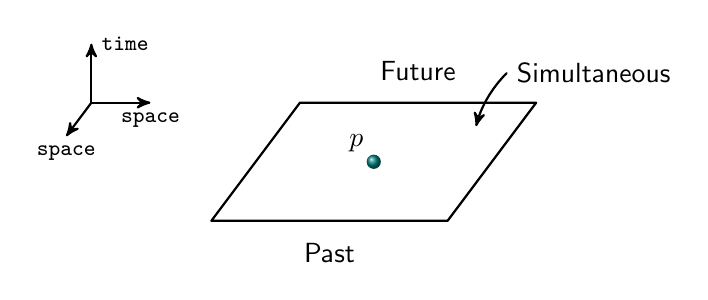
\begin{tikzpicture}[scale=1.5]
        \draw [->, xshift=-.4in] (0,1) -- (.5,1) node [anchor=north] {\ttfamily\footnotesize space};
        \draw [->, xshift=-.4in] (0,1) -- (0,1.5) node [anchor=west] {\ttfamily\footnotesize time};
        \draw [->, xshift=-.4in] (0,1) -- ({-.3/sqrt(2)},{1-.4/sqrt(2)}) node [anchor=north] {\ttfamily\footnotesize space};
        \draw [thick] (0,0) -- (2,0) node [midway,anchor=north, yshift=-1ex] {\sffamily Past} -- (2.75,1) -- (.75,1) node [midway,anchor=south, yshift=1ex] {\sffamily Future} -- cycle;
        \shade [ball color=teal] (1.375,.5) circle (.06) node [anchor=south east] {$p$};
        \draw [->] (2.5,1.25) arc (135:165:1) node [anchor=west,at start] {\sffamily Simultaneous};
    \end{tikzpicture}
\end{minipage}
\hfill
\begin{minipage}{.32\textwidth}
    \caption{A diagram showing the causal structure of spacetime in prerelativity physics. Given an event $p$, all other events in spacetime either are to the future of $p$, to the past of $p$, or Simultaneous with $p$. The simultaneous events form a three-dimensional surface in spacetime.}
    \label{1.1}
\end{minipage}
\end{figure}

In prerelativity physics, events in the third category are assumed to form a three-dimensional set and define the notion of simultaneity with $p$, as is illustrated in \figref{1.1}.

The belief that the causal structure of spacetime has the character shown in \figref{1.1} turns out to be wrong. In special relativity theory the above classification of the causal relationships between events still holds. The crucial difference is that events in category (3) form more than a three-dimensional set; the causal relation between $p$ and other events has the structure sketched in \figref{1.2}. The events in category (3) can be further subdivided as follows
\begin{itemize}
    \item Events that lie on the boundary of the set of points to the future of $p$. These events cannot be reached by a material particle starting at $p$ but can be reached by a light signal emitted from p. They form the ``future light cone'' of $p$ (a three-dimensional set).
    \item Events on the past light cone of $p$, defined similarly.
    \item Events in category (3) which are on neither the past nor the future light cone. These events are said to be spacelike related to $p$ and comprise a four-dimensional set.
\end{itemize}
    
A key fact closely related to the above is that in special relativity there is no notion of absolute simultaneity; there are no absolute three-dimensional surfaces in space-time as in \figref{1.1}. As we shall see below, an observer still can define a notion of which events occur ``at the same time'' as a given event-thus defining a three-dimensional surface in spacetime—but the notion he gets depends upon his state of motion. (On the other hand, the light cones of \figref{1.2} \emph{are} absolute surfaces.) The notion that there is absolute simultaneity is a deeply ingrained one. The fact that there is no such notion is one of the most difficult ideas to adjust to in the theory of special relativity.

\begin{figure}[!ht]
\begin{minipage}{.32\textwidth}
    \caption{A diagram showing the causal structure of spacetime in special relativity. The ``light cone'' of $p$ rather than a ``surface of simultaneity'' with $p$ now plays a fundamental role in determining the causal relationship of $p$ to other events.}
    \label{1.2}
\end{minipage}
\hfill
\begin{minipage}{.64\textwidth}
    \centering
    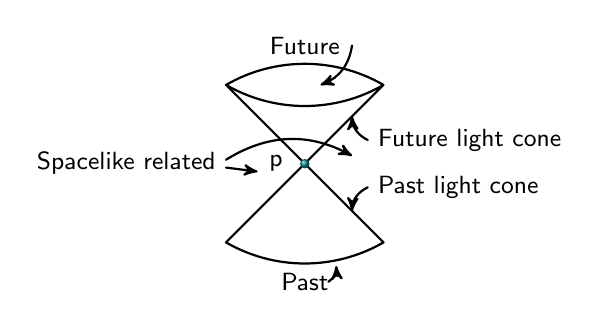
\begin{tikzpicture}
        \draw [line join=round,line cap=round] (-1,1) -- (1,-1) arc (-60:-120:2) -- (1,1) arc (-60:-120:2) arc (-60:-120:-2);
        \shade [ball color=teal] (0,0) circle (.06) node [anchor=east,xshift=-1ex] {\sffamily\small p};
        \node at (0,1.5) {\sffamily\small Future};
        \path [->] (.6,1.5) edge [bend left] (.2,1);
        \node at (0,-1.5) {\sffamily\small Past};
        \path [->] (.3,-1.5) edge [bend right] (.4,-1.3);
        \node [left] at (-1,0) {\sffamily\small Spacelike related};
        \path [->] (-1,-.05) edge (-.6,-.1);
        \path [->] (-1,.05) edge [bend left] (.6,.1);
        \node [right] at (.8,.3) {\sffamily\small Future light cone};
        \path [->] (.8,.3) edge [bend left] (.6,.6);
        \node [right] at (.8,-.3) {\sffamily\small Past light cone};
        \path [->] (.8,-.3) edge [bend right] (.6,-.6);
    \end{tikzpicture}
\end{minipage}
\end{figure}

In special relativity (as in prerelativity physics) one has the notion of inertial, ``nonaccelerating'' motion, namely the motion a material body would undergo if subjected to no external forces. An inertial observer can label the events of spacetime in the following manner. He can build himself a rigid frame and label the grid points of the frame with the Cartesian coordinates $x, y, z$ of the (assumed Euclidean) geometry of the frame. He can then have a clock placed at each grid point and can synchronize each clock with his by a symmetrical procedure, e.g., by making sure that a given clock and his give the same reading when they receive a signal sent out in a symmetrical manner by an observer stationed halfway between the two. (Because the causal structure of spacetime is that of \figref{1.2}, not \figref{1.1}, synchronization is not a trivial issue.) The observer may carry the grid, complete with synchronized clocks, in a nonrotating manner. Each event in spacetime can now be labeled with the coordinates $x, y, z$ of the grid point at which the event occurred and the reading $t$ of the (synchronized) clock at that event. The labels $t, x, y, z$ assigned to events in this manner are referred to as global inertial coordinates. 

If two such inertial observers go through this procedure, one may compare the coordinate labels they assign to events. In prerelativity physics (where the same labeling procedure works, the only difference being that clock synchronization \emph{is} trivial), if observer $O$ labels an event $p$ with coordinates $t, x, y, z$ and $O'$ moves with velocity $\vv{v}$ in the $x$-direction, passing observer $O$ at the event labeled $t = x = y = z = 0$. the coordinate labels that $O'$ assigns to event $p$ are

\begin{align}
    & t'=t\label{1.2.1}\\
    & x'=x-vt\label{1.2.2}\\
    & y'=y\label{1.2.3}\\
    & z'=z\label{1.2.4}
\end{align}

In special relativity, however, the labeling by $O'$ will be related that of $O$ by a Lorentz transformation
\begin{align}
    & t'=(t-vx/c^2)/(1-v^2/c^2)^{1/2}\label{1.2.5}\\
    & x'=(x-vt)/(1-v^2/c^2)^{1/2}\label{1.2.6}\\
    & y'=y\label{1.2.7}\\
    & z'=z\label{1.2.8}
\end{align}

where $c$ is the speed of light. \eqref{1.2.5} shows that the notion of simultaneity determined by $O$ (namely, $t = \text{constant}$) differs from that determined by $O'$ ($t' = \text{constant}$), as illustrated in \figref{1.3}.

\begin{figure}[!ht]
    \centering
    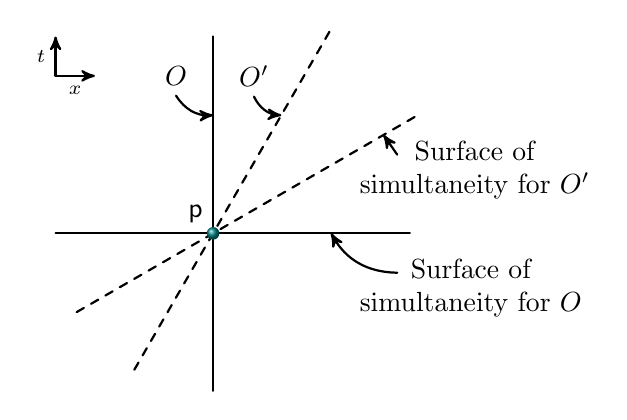
\begin{tikzpicture}
        \draw [->, xshift=-2 cm,yshift=2 cm] (0,0) -- (.5,0) node [anchor=north,midway] {$\scriptstyle x$};
        \draw [->, xshift=-2 cm, yshift=2 cm] (0,0) -- (0,.5) node [anchor=east,midway] {$\scriptstyle t$};
        \draw [thick] (-2,0) -- (2.5,0);
        \draw [thick] (0,-2) -- (0,2.5);
        \draw [dashed] ({-sqrt(3)},-1) -- ({3*sqrt(3)/2},1.5);
        \draw [dashed] (-1,{-sqrt(3)}) -- (1.5,{3*sqrt(3)/2});
        \shade [ball color=teal] (0,0) circle (.08) node [anchor=south east] {\sffamily p};
        \node [align = center,right] at ({sqrt(3)},.8) {Surface of\\simultaneity for $O'$};
        \draw [->] ({1.35*sqrt(3)},1) -- ({5*sqrt(3)/4},1.25);
        \node [align = center,below right] at ({sqrt(3)},-.2) {Surface of\\simultaneity for $O$};
        \path [->] ({1.35*sqrt(3)},-.5) edge [bend left] (1.5,0);
        \node [left] (O) at (-.2,2) {$O$};
        \path [->] (O.south) edge [bend right] (0,1.5);
        \node [right] (O') at (.2,2) {$O'$};
        \path [->] (O'.south) edge [bend right] ({sqrt(3)/2},1.5);
    \end{tikzpicture}
    \caption{A spacetime diagram illustrating the fact that in special relativity the inertial observers $O$ and $O'$ disagree over the definition of simultaneity with event $p$.}
    \label{1.3}
\end{figure}

\section{The Spacetime Metric}

In the previous section, we gave a prescription for how an inertial observer $O$ can label the events in spacetime with global inertial coordinates $t, x, y, z$. However, a fundamental tenet of special relativity is that there are no preferred inertial observers. As seen above. a different inertial observer using the same procedure assigns different labels $t',x',y',z'$ to the events in spacetime. Thus, the coordinate labels themselves do not have intrinsic significance since they depend as much on which observe does the labeling as they do on the properties of spacetime itself. It is of great interest to determine what quantities have absolute, observe-independent significance, i.e., truly measure intrinsic structure of spacetime. This is equivalent to determining what functions of global inertial coordinates are independent of the choice of inertial frame.

In prerelativity physics the answer is the following. The time interval $\Delta t$ between two events has absolute significance; all observers will agree on the value of $\Delta t$. Furthermore, the spatial interval $\abs{\Delta\vv{x}}$ between two simultaneous events is observer independent. However, these quantities (or functions of them) are the only ones with absolute significance. For example, observers moving with nonzero relative velocity will disagree over the spatial interval between nonsimultaneous events. In special relativity neither the time interval nor the space interval between ``relatively simultaneous'' events (i.e., events determined to be simultaneous by a particular observer) has absolute significance. The quantity which is observer independent is the spacetime interval, $I$, defined by
\begin{equation}
    I=-(\Delta t)^2+\frac{1}{c^2}\ab[(\Delta x)^2+(\Delta y)^2+(\Delta z)^2]
    \label{1.3.1}
\end{equation}

Indeed, the Poincaré transformations (the set of all possible transformations between global inertial coordinates) consist precisely of the linear transformations which leave $I$ unchanged. The spacetime interval $I$ and functions of $I$ are the only observer-independent quantities characterizing the spacetime relationships between events.

What is truly remarkable about the expression for $I$ is that it is quadratic in the coordinate differences, just like the distance function in Euclidean (i.e., flat, positive definite) geometry. Indeed, the only difference is the minus sign in front of $(\Delta t)^2$, allowing $I$ to become zero or negative. We shall refer to $I$ as the metric of spacetime in analogy to an ordinary Euclidean metric. (More precisely, the metric of spacetime in special relativity will be defined later to be a tensor field associated with the formula for the spacetime interval between two ``infinitesimally nearby'' events; see \eqref{4.2.2} below.) As we shall see in chapter 3, this difference in metric signature makes very little difference in the mathematical analysis of metrics. In particular definitions of geodesics (``straightest possible lines'') and curvature carry through in the same way for metrics with the signature of $I$ as for ordinary positive definite metrics. It is interesting to note that, as discussed more fully in chapter 4, the paths in spacetime of inertial observers in special relativity are geodesics of the spacetime metric, and the curvature associated with $I$ is zero, i.e., the spacetime geometry in special relativity is flat.

\section{General Relativity}
Prior to special relativity, the prerelativity notions of space and time pervaded-among many other things-the formulation of the laws of physics. When these notions were overthrown, the task remained of modifying and reformulating physical laws to be consistent with the spacetime structure given by the theory of special relativity. Maxwell's theory of electromagnetism was already consistent with special relativity. Indeed, its incompatibility with prerelativity notions of spacetime structure unless preferred inertial frames were introduced led directly to the discovery of special relativity. Newton's theory of gravitation is not consistent with special relativity since it invokes notions of instantaneous influence of one body on another, but it might be thought that one could simply modify it to fit within the framework of special relativity.

However, two key ideas motivated Einstein \emph{not} to follow this path but rather to seek an entirely new theory of spacetime and gravitation-a theory that revolutionized our notions of space and time every bit as much as special relativity already had done.

The first idea is that \emph{all} bodies are influenced by gravity and, indeed, all bodies fall precisely the same way in a gravitational field. This fact, known as the \emph{equivalence principle}, is expressed in the Newtonian theory of gravitation by the statement that the gravitational force on a body is proportional to its inertial mass. Because motion is independent of the nature of the bodies, the paths of freely falling bodies define a preferred set of curves in spacetime just as in special relativity the paths in spacetime of inertial bodies define a preferred set of curves, independent of the nature of the bodies. This suggests the possibility of ascribing properties of the gravitational field to the structure of spacetime itself. As already mentioned in the previous section, the paths of inertial bodies in special relativity are geodesics of the spacetime metric. Perhaps, then, the paths of freely falling bodies are always geodesics, but the spacetime metric is not always that given by special relativity. What we think of as a gravitational field would then not be a new field at all, but rather would correspond to a deviation of the spacetime geometry from the flat geometry of special relativity. We shall discuss these ideas further in chapter 4.

The second much less precise set of ideas which motivated the formulation of general relativity goes under the name of \emph{Mach's principle}. In special relativity as in prerelativity notions of spacetime, the structure of spacetime is given once and for all and is unaffected by the material bodies that may be present. In particular, ``inertial motion'' and ``nonrotating'' are not influenced by matter in the universe. Mach as well as a number of earlier philosophers and scholars (in particular, Riemann) found this idea unsatisfactory. Rather, Mach felt that all matter in the universe should contribute to the local definition of ``nonaccelerating'' and ``nonrotating''; that in a universe devoid of matter there should be no meaning to these concepts. Einstein accepted this idea and was strongly motivated to seek a theory where, unlike special relativity, the structure of spacetime is influenced by the presence of matter.

The new theory of space, time, and gravitation-general relativity-proposed by Einstein states the following: The intrinsic, observer-independent, properties of spacetime are described by a spacetime metric, as in special relativity. However, the spacetime metric need not have the (flat) form it has in special relativity. Indeed, curvature, i.e., the deviation of the spacetime metric from flatness, accounts for the physical effects usually ascribed to a gravitational field. Furthermore, the curvature of spacetime is related to the stress-energy-momentum tensor of the matter in spacetime via an equation postulated by Einstein. In this way, the structure of spacetime (as embodied in the spacetime metric) is related to the matter content of spacetime, in accordance with some (but not all!) of Mach's ideas. Thus far, the predictions of general relativity have been found to be in excellent agreement with experiments and observations (see section 6.3 below and Will 1981).

Most of the remainder of this book is devoted to exploring the consequences of this theory. Our first task, however, is to give a precise, mathematical expression to the ideas discussed in this chapter. To begin with, we must give a precise formulation of the notion that spacetime is a four-dimensional continuum. This will be accomplished with the definition of a manifold given in section 2.1. We must then introduce the basic mathematical framework needed to discuss curved geometry: vectors and tensors (2.2), the metric (2.3), derivative operators (3.1), curvature (3.2), and geodesics (3.3). Almost all of the discussion we shall give applies equally well to the differential geometry of ordinary surfaces (positive definite metric) as to the geometry of spacetime (metric of Lorentz signature). After development of these mathematical tools and techniques, we will then be in position to begin our study of general relativity in chapter 4.

\begin{problem}
    \emph{Car and garage paradox}: The lack of a notion of absolute simultaneity in special relativity leads to many supposed paradoxes. One of the most famous of these involves a car and a garage of equal proper length. The driver speeds toward the garage, and a doorman at the garage is instructed to slam the door shut as soon as the back end of the car enters the garage. According to the doorman, ``the car Lorentz contracted and easily fitted into the garage when I slammed the door.'' According to the driver, ``the garage Lorentz contracted and was too small for the car when I entered the garage.'' Draw a spacetime diagram showing the above events and explain what really happens. Is the doorman's statement correct? Is the driver's statement correct? For definiteness, assume that the car crashes through the back wall of the garage without stopping or slowing down.
\end{problem}

\begin{solution}

Let $c=1$. The spacetime diagram can be found below. In it the primed coordinates are those assigned to events by the driver and the unprimed ones are those assigned by the doorman. At the origin is the event ``the driver has just reached the doorman and is about to enter the garage''. It follows that the world lines of the driver and doorman are the $t'$-axis and the $t$-axis, respectively.

Let $L$ denote the common proper length of the car and the garage. The world line of the back wall of the garage is thus the one parallel to the $t$-axis and passing through the point $(x,t)=(L,0)$. Similarly, the world line of the rear end of the car is the one parallels to the $t'$-axis and passing through $(x',t')=(-L,0)$.

\columnratio{.32}
\begin{paracol}{2}
    \begin{center}
    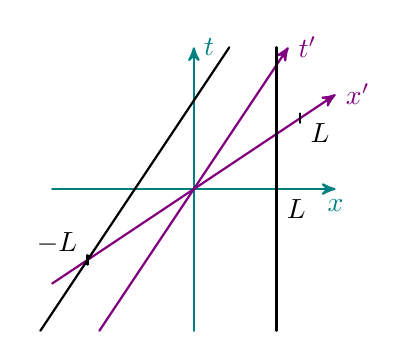
\begin{tikzpicture}[scale=.6]
        \draw [->,teal] (-3,0) -- (3,0) node [below] {$x$};
        \draw [->,teal] (0,-3) -- (0,3) node [right] {$t$};
        \draw [->,violet] (-2,-3) -- (2,3) node [right] {$t'$} ;
        \draw [->,violet] (-3,-2) -- (3,2) node [right] {$x'$} ;
    
        \draw [xshift=-1.25 cm] (-2,-3) -- (2,3);
        \draw [thick] (-2.25,-1.4) -- (-2.25,-1.6) node [above left] {$-L$};
        \draw [thick] (2.25,1.4) -- (2.25,1.6) node [below right] {$L$};
    
        \draw [thick] (1.75,3) -- (1.75,-3) node [midway, below right] {$L$};
    \end{tikzpicture}
    \end{center}
    \switchcolumn
    Analyzing the spacetime diagram, one concludes that both statements are correct.

    The intersection of the $t' = 0$ line with the world line of the back wall of the garage is at a smaller value of $x'$ than $L$. This agrees with the driver's account.
        
    Let $t_\text{slam}$ be time coordinate recorded by the doorman as he slams the door shut. This event is at the intersection of the world lines of the doorman and that of the car's rear end. The line $t = t_\text{slam}$ intersects the world line of the driver at a smaller value of $x$ than that of the back wall of the garage. This agrees with the doorman's statement.
\end{paracol}

So what happens here? The driver is correct to say he had crashed through the back wall of the garage by the time the doorman shuts the door. The doorman is also correct when he says the back wall was intact by the time he closed the door. This seems to be a contradiction since from both statements one would conclude that the car would and would have not crashed by the time the door was closed. It turns out this conclusion would be wrong. This is because the expression ``by the time the door was closed'' means different things to the driver and the doorman. To the driver, it refers to a line parallel to the $x'$-axis. To the doorman, the expression refers to those events in a line parallel to the $x$-axis.
\end{solution}
\chapter{Manifols and Tensor Fiels}
In this chapter we lay the foundations for a precise, mathematical formulation of general relativity by obtaining some basic properties of manifols and tensor fiels. As defined in section 2.1, an $n$-dimensional manifold is a set that has the local differential structure of $\mathbb{R}^n$ but not necessarily its global properties. In section 2.2 we define tangent vectors as directional derivative operators acting on functions defined on a manifold. We obtain there some important properties of coordinate bases of the tangent space and tangents to curves. Tensors are introduced in section 2.3, and the notion of a metric is defined. Finally, in section 2.4 we introduce the abstract index notation for tensors, which we shall use throughout the remainder of this book. We will use a fair number of standard mathematical symbols in this chapter, and the reader unfamiliar with these symbols should consult the section ``Notation and Conventions'' at the beginning of this book.

\section{Manifols}
As mentioned in the previous chapter, our experience tells us that spacetime is a ``four-dimensional continuum'' in the sense that it requires four numbers to characterize an event. In prerelativity physics as well as in special relativity it is assumed that this is globally true, i.e., that all events in spacetime can be put into one-to-one continuous correspondence with the points of $\mathbb{R}^4$. However, in general relativity we will be solving for the spacetime geometry and we do not wish to prejudice in advance any aspects of the global nature of spacetime structure. Our situation is very similar to that of hypothetical investigators of the structure of the surface of Earth prior to the explorations of Columbus and Magellan. Such investigators might notice that in their vicinity they can characterize positions on the surface of the Earth by two numbers. However, they would be making a serious error is they were to extrapolate from this fact to the conclusion that the entire collection of points on the surface of the Earth can be put into one-to-one correspondence with points of $\mathbb{R}^2$ in a continuous manner. Thus, what is needed as a mathematical basis for beginning the investigation of spacetime structure (as well as the surface of the Earth) is a precise notion of a manifold, that is, a set in which the vicinity of every point ``looks like'' $\mathbb{R}^n$ but which may have quite different global properties.

In the case of the Earth, our investigators might be aware that its surface ``lives'' in the higher dimensional Euclidean space $\mathbb{R}^3$ of all space points (at least, according to prerelativity notions of space and time). Thus the study of two-dimensional surfaces embedded in  $\mathbb{R}^3$ would provide an adequate mathematical framework to analyze the structure of the Earth's surface, and one could avoid making an abstract definition of manifols. However, in general relativity, spacetime itself does not (as far as we know) naturally live in a higher dimensional Euclidean space, so an abstract definition is much more natural. Indeed, such a definition turns out to be extremely useful even for the study of ordinary surfaces in $\mathbb{R}^3$.

Before defining the notion of a manifold we remind the reader that an \emph{open ball} in $\mathbb{R}^n$ of radius $r$ centered around point $y=(y^1,\ldots,y^n)$ consists of the points $x$ such that $\abs{x-y}<r$, where

\[\textstyle\abs{x-y}=\ab[\sum_{\mu=1}^n(x^\mu-y^\mu)^2]^{1/2}\]

An \emph{open set} in $\mathbb{R}^n$ is any set which can be expressed as a union of open balls. This notion of open set makes $\mathbb{R}^n$ a topological space in the sense discussed in appendix A.

Basically, a \emph{manifold} is a set made up of pieces that ``look like'' open subsets of $\mathbb{R}^n$ such that these pieces can be ``sewn together'' smoothly. More precisely, an \emph{$n$-dimensional}, $C^\infty$, \emph{real manifold $M$} is a set together with a collection of subsets $\{O_\alpha\}$ satisfying the following properties
\begin{enumerate}[label=(\arabic*)]
    \item Each $p\in M$ lies in at least one $O_\alpha$, i.e., the $\{O_\alpha\}$ cover $M$.
    \item For each $\alpha$, there is a one-to-one, onto, map $\psi_\alpha:\ O_\alpha\to U_\alpha$, where $U_\alpha$ is an open subset of $\mathbb{R}^n$.
    \item If any two sets $O_\alpha$ and $O_\beta$ overlap, $O_\alpha\cap O_\beta\neq\varnothing$ (where $\varnothing$ denotes the empty set), we can consider the map $\psi_\beta\circ\psi_\alpha^{-1}$ (where $\circ$ denotes composition) which takes points in $\psi_\alpha[O_\alpha\cap O_\beta]\subset U_\alpha\subset\mathbb{R}^n$ to points in $\psi_\beta[O_\alpha\cap O_\beta]\subset U_\beta\subset\mathbb{R}^n$ (see \figref{2.1}). We require these subsets of $\mathbb{R}^n$ to be open and this map to be $C^\infty$, i.e., infinitely continuously differentiable. (Since we are dealing here with maps of $\mathbb{R}^n$ into $\mathbb{R}^n$, the advanced calculus notion of $C^\infty$ functions applies.)
\end{enumerate}

Each map $\psi_\alpha$ is generally called a \emph{chart} by mathematicians and a \emph{coordinate system} by physicists. We shall use these terms interchangeably. In order to prevent one from defining new manifolds by merely deleting or adding in a coordinate system, it is convenient also to require in the definition of $M$ that the cover $\{O_\alpha\}$ and chart family $\{\psi_\alpha\}$ is maximal, i.e., all coordinate systems compatible with (2) and (3) are included. The definition of $C^k$ or analytic manifolds is the same as above with the appropriate change in requirement (3). To define a complex manifold, one merely replaces $\mathbb{R}^n$ by $\mathbb{C}^n$ above.

\begin{figure}[!ht]
    \centering
    \begin{tikzpicture}
        \node [inner sep=0pt] at (0,0) {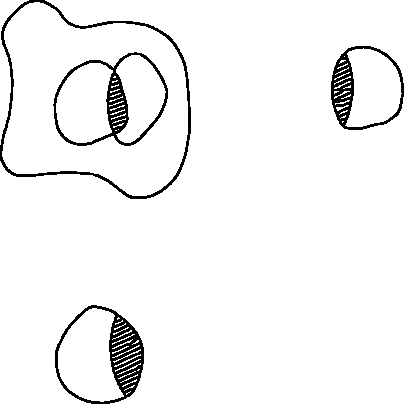
\includegraphics{fig2.1}};
        \node at (-2.75,2.75) {$\scriptstyle\mathsf{M}$};
        \node at (-2,1.75) {$\scriptstyle O_\alpha$};
        \node at (-1,1.75) {$\scriptstyle O_\beta$};
        \draw (-2.875,-1.25) rectangle (-.625,-3.75) node [at start, below right] {$\scriptstyle\mathsf{R}^n$};
        \draw (1.5,3) rectangle (3.75,.75) node [at start, below right] {$\scriptstyle\mathsf{R}^n$};
        \draw [->] (-2,1.5) -- (-2,-2.5) node [midway,right] {$\scriptstyle\psi_\alpha$} node [below] {$\scriptstyle U_\alpha$};
        \draw [->] (-.8,1.9) -- (2.8,1.9) node [midway,above] {$\scriptstyle\psi_\beta$} node [right] {$\scriptstyle U_\beta$};
        \draw [->] (-1.25,-2.5) -- (2.5,1.75) node [midway,above,sloped] {$\scriptstyle\psi_\beta\circ\psi_\alpha^{-1}$};
    \end{tikzpicture}
    \caption{An illustration of the map $\psi_\beta\circ\psi_\alpha^{-1}$ arising when two coordinate systems overlap.}
    \label{2.1}
\end{figure}
 
We can define a topology on the manifold $M$ by demanding that all the maps $\psi_\alpha$ in our maximal collection be homeomorphisms (see appendix A for definitions). Indeed, it is perhaps more natural to proceed by defining a manifold to be a topological space satisfying the above properties, with each $\psi_\alpha$ a homeomorphism. (We have not done so simply in order to avoid introducing the machinery of topological spaces in the main text.) Viewed as topological spaces, we shall consider in this book only manifolds which are \emph{Hausdorff} and \emph{paracompact}; these terms are explained in appendix A.

Euclidean space $\mathbb{R}^n$ provides a trivial example of a manifold, which can be covered by a single chart ($O=\mathbb{R}^n$, $\psi=\text{identity map}$). A more interesting example of a manifold is the $2$-sphere $S^2$
 \[S^2=\ab\{\ab(x^1,x^2,x^3)\in\mathbb{R}|\ab(x^2)^2+\ab(x^2)^2+\ab(x^3)^2=1\}\]

The entire $2-$sphere $S^2$ cannot be mapped into $\mathbb{R}^2$ in a continuous, $1-1$ manner, but ``pieces'' of $S^2$ can, and these can be ``smoothly sewn together''. For example, if we define the six hemispherical open sets $O_i^\pm$ for $i=1,2,3$ by
\[
    O_i^\pm=\ab\{\ab(x^1,x^2,x^3)\in S^2|\pm x^i>0\}
\]

then $\ab\{O_i^\pm\}$ covers $S^2$. Furthermore, each $O_i^\pm$ can be mapped homeomorphically into the open disk $D=\ab\{(x,y)\in\mathbb{R}^2|x^2+y^2<1\}$ in the plane via the ``projection maps'' $f_1^+:O_1^+\to D$, $f_1^-:O_1^-\to D$, etc., defined by $f_1^+(x^1,x^2,x^3)=(x^2,x^3)$, etc. The overlap functions $f_i^\pm\circ(f_j^\pm)^{-1}$ can be checked to be $C^\infty$ in their domain of definition (problem 1). Thus, $S^2$ is a two-dimensional manifold. In a similar manner, the $n$-dimensional sphere $S^n$ is seen to be a manifold.

Given two manifolds $M$ and $M'$ of dimension $n$ and $n'$, respectively, we can make the product space $M\times M'$ consisting of all pairs $(p,p')$ with $p\in M$ and $p'\in M'$ into an $(n+n')$-dimensional manifold as follows. If $\psi_\alpha:O_\alpha\to U_\alpha$ and $\psi_\beta':O_\beta'\to U_\beta'$ are charts, we define a chart $\psi_{\alpha\beta}:O_{\alpha\beta}\to U_{\alpha\beta}\subset\mathbb{R}^{n+n'}$ on $M\times M'$ by taking $O_{\alpha\beta}=O_\alpha\times O_\beta'$, $U_{\alpha\beta}=U_\alpha\times U_\beta'$, and setting $\psi_{\alpha\beta}(p,p')=[\psi_\alpha(p),\psi_\beta'(p')]$. it is easily checked that the chart family $\{\psi_{\alpha\beta}\}$ satisfies the properties required to define a manifold structure on $M\times M'$. Most manifolds we will consider in this book can be expressed as products of Euclidean space $\mathbb{R}^n$ with spheres $S^m$.

With the structure on manifolds given by the coordinate systems, we may now define the notion of differentiability and smoothness of maps between manifolds. Let $M$ and $M'$ be manifolds and let $\{\psi_\alpha\}$ and $\{\psi_\beta'\}$ denote the chart maps. A map $f:M\to M'$ is said to be $C^\infty$ if for each $\alpha$ and $\beta$, the map $\psi_\beta'\circ f\circ\psi_\alpha^{-1}$ taking $U_\alpha\subset\mathbb{R}^n$ into $U_\beta'\subset\mathbb{R}^n$ is $C^\infty$ inverse, $f$ is called a \emph{diffeomorphism} and $M$ and $M'$ are said to be \emph{diffeomorphic}. Diffeomorphic manifolds have identical manifold structure.

\section{Vectors}
The concept of a vector space is undoubtedly familiar to most readers. In prerelativity physics it is assumed that space has the natural structure of a three-dimensional vector space once one has designated a point to serve as the origin; the natural rules for adding and scalar multiplying spatial displacements satisfy the vector space axioms\footnote{See, e.g., Royden (1963) for the list of vector space axioms.}. In special relativity, spacetime similarly has the natural structure of a four-dimensional vector space. However, when one considers curved geometries (as we do in general relativity), this vector space structure is lost. For example, there is no natural notion of how to ``add'' two points on a sphere and end up with a third point on the sphere. Nevertheless, vector space structure can be recovered in the limit of ``infinitesimal displacements'' about a point. It is this notion of ``infinitesimal displacements'' or tangent vectors which lies at the foundation of calculus on manifolds. Therefore, we will devote considerable attention below to giving a precise mathematical definition of this concept.

For manifolds like the sphere, which arise naturally as surfaces embedded in $\mathbb{R}^n$ the intuitive notion of a tangent vector at point $p$ is a vector lying in the tangent plane illustrated in \figref{2.2}. For manifolds embedded in $\mathbb{R}^n$, this idea can be made mathematically precise. However, in many situations-most importantly in general relativity-one is given a manifold without an embedding of it in $\mathbb{R}^n$. Thus, it is important (and, in the long run, much more useful) to define a tangent vector in a way that refers only to the intrinsic structure of the manifold, not to its possible embeddings in $\mathbb{R}^n$.

\begin{figure}[!ht]
\centering
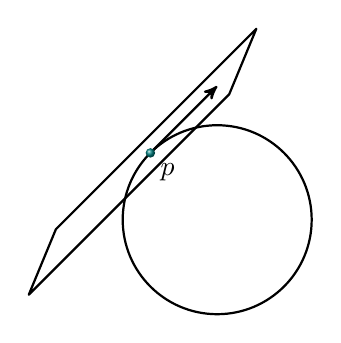
\begin{tikzpicture}
    \draw (0,0) circle (1.2);
    \draw [->] ({-1.2/sqrt(2)},{1.2/sqrt(2)}) --++ ({1.2/sqrt(2)},{1.2/sqrt(2)}) node [at start,below right] {$p$};
    \shade [ball color=teal] ({-1.2/sqrt(2)},{1.2/sqrt(2)}) circle (.06);
    \draw [xshift=(-1.2/sqrt(2)-1.2)*1cm,yshift=(-1.2/sqrt(2)+0.9-0.45*cos(22.5)+0.45*sin(22.5)/sin(45))*1cm] (0,0) -- ({1.8*sqrt(2)},{1.8*sqrt(2)}) --++ ({-.9*sin(22.5)},{-.9*cos(22.5)}) --++ ({-1.8*sqrt(2)},{-1.8*sqrt(2)}) -- cycle;
\end{tikzpicture}
\caption{The tangent plane at point $p$ of a sphere in $\mathbb{R}^3$.}
\label{2.2}
\end{figure}

Such a definition is provided by the notion of a tangent vector as a directional derivative. In $\mathbb{R}^n$ there is a one-to-one correspondence between vectors and directional derivatives. A vector $v=(v^1,\ldots,v^n)$ defines the directional derivative operator $\sum_\mu v^\mu(\partial/\partial x^\mu)$ and vice versa. Directional derivatives are characterized by their linearity and ``Leibnitz rule'' behavior when acting on functions. Thus on a manifold $M$ let $\mathscr{F}$ denote the collection of $C^\infty$ functions from $M$ into $\mathbb{R}$. We define a tangent vector $v$ at point $p\in M$ to be a map $v:\mathscr{F}\to\mathbb{R}$ which (1) is linear and (2) obeys the Leibnitz rule
\begin{enumerate}[label=(\arabic*)]
    \item $v(af+bg)=av(f)+bv(g)$, for all $f$, $g\in\mathscr{F}$; $a$, $b\in\mathbb{R}$.
    \item $v(fg)=f(p)v(g)+g(p)v(f)$.
\end{enumerate}

Note that (1) and (2) imply that if $h\in\mathscr{F}$ is a constant function. i.e., $h(q)=c$ for all $q\in M$, then $v(h)=0$, since from (2) we have $vv{v}(h^2)=2cv(h)$ whereas from (1) we have $v(h^2)=v(ch)=cv(h)$.

Though it may not be obvious at first glance, this definition does indeed make precise and give intrinsic meaning to the concept of an ``infinitesimal displacement''. In the first place, it is easy to see that the collection, $V_p$, of tangent vectors at $p$ has the structure of a vector space under the addition law $(v_1+v_2)(f)=v_1(f)+v_2(f)$ and scalar multiplication law $(av)(f)=av(f)$. A second vital property of $V_p$, is given by the following theorem

\begin{theorem}
    \itshape Let $M$ be an $n$-dimensional manifold. Let $p\in M$ and let $V_p$ denote the tangent space at $p$. Then $\dim V_p=n$.
\end{theorem}
\begin{figure}[!ht]
\centering
\begin{tikzpicture}
    \node at (0,0) {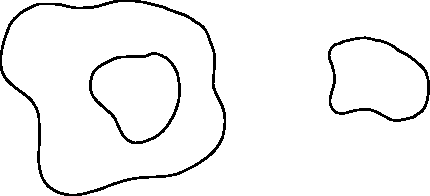
\includegraphics{fig2.3.pdf}};
    \draw [semithick] (1.25,1.75) rectangle (3.75,-1.25) node [at start,below right] {$\scriptstyle\mathsf{R}^n$};
    \draw [<->,semithick] (1.75,-.25) -- (1.75,-.75) node [at start,left,xshift=.25em] {$\scriptstyle x^2$} -- (2.25,-.75) node [below,yshift=.25em] {$\scriptstyle x^1$};
    \draw [->,semithick] (-.75,.25) -- (2.5,.25) node [above] {$\scriptstyle U$} node [midway,above] {$\scriptstyle\psi$};
    \shade [ball color=teal] (-1,.25) circle (.06) node [left] {$\scriptstyle p$};
    \shade [ball color=teal] (2.5,.125) circle (.06) node [right] {$\scriptstyle\psi(p)$};
    \draw [->,semithick] (-1,-.25) -- (-1,-4) node [at start,left] {$\scriptstyle O$} node [midway,right] {$\scriptstyle f$};
    \draw [semithick] (-4,-4) -- (0,-4) node [above left] {$\scriptstyle\mathsf{R}$};
\end{tikzpicture}
\caption{A diagram illustrating the definition of the directional derivatives $X_\mu$, used in theorem 2.2.1.}
    \label{2.3}
\end{figure}
\begin{proof}
    We shall show that $\dim V_p=n$ by constructing a basis of $V_p$, i.e., by finding $n$ linearly independent tangent vectors which span $V_p$. Let $\psi:O\to U\subset\mathbb{R}^n$ be a chart with $p\in O$ (see \figref{2.3}). If $f\in\mathscr{F}$, then by definition $f\circ\psi^{-1}:U\to\mathbb{R}$ is $C^\infty$. For $\mu=1,\ldots,n$ define $X_\mu:\mathscr{F}\to\mathbb{R}$ by
\begin{equation}
    X_\mu(f)=\pdv{}{X^\mu}(f\circ\psi^{-1})\bigg|_{\psi(p)}
\end{equation}

where $(x^1,\ldots,x^n)$ are the Cartesian coordinates of $\mathbb{R}^n$. Then $X_1,\ldots,X_n$ are tangent vectors, and it is easily seen that they are linearly independent. To show that they span $V_p$ we make use of the following result from advanced calculus (see problem 2): If $F:\mathbb{R}^n\to\mathbb{R}$ is $C^\infty$, then for each $a=(a^1,\ldots,a^n)\in\mathbb{R}^n$ there exists $C^\infty$ functions $H_\mu$ such that for all $x\in\mathbb{R}^n$ we have
\begin{equation}
    F(x)=F(a)+\sum_{\mu=1}^n(x^\mu-a^\mu)H_\mu(x)
    \label{2.2.2}
\end{equation}

Furthermore, we have
\begin{equation}
    H_\mu(a)=\pdv{F}{x^\mu}\bigg|_{x=a}
    \label{2.2.3}
\end{equation}

We apply this result here, letting $F=f\circ\psi^{-1}$ and $a=\psi(p)$. Then, for all $q\in O$ we have
\begin{equation}
    f(q)=f(p)+\sum_{\mu=1}^n\ab[x^\mu\circ\psi(q)-x^\mu\circ\psi(p)]H_\mu(\psi(q))
    \label{2.2.4}
\end{equation}

Let $v\in V_p$. We wish to show that $v$ is a linear combination of $X_1,\ldots,X_n$. To do so, we apply $v$ to $f$, using \eqref{2.2.4}, the linearity and Leibnitz properties of $v$, and the fact that $v$ applied to a constant [such as $f(p)$] vanished. We obtain
\begin{equation}
\begin{aligned}
    f(q)= & f(p)+\sum_{\mu=1}^n\Bigg\{\ab[x^\mu\circ\psi(q)-x^\mu\circ\psi(p)]\bigg|_{q=p}v(H_\mu\circ\psi)\\
    & +(H_\mu\circ\psi)\bigg|_pv\ab[x^\mu\circ\psi-x^\mu\circ\psi(p)]\Bigg\}\\
    = & \sum_{\mu=1}^n[H_\mu\circ\psi(p)]v(x^\mu\circ\psi)
\end{aligned}
\label{2.2.5}
\end{equation}

But by \eqref{2.2.3}, $H_\mu\circ\psi(p)$ is just $X_\mu(f)$. Thus, for all $f\in\mathscr{F}$, we have
\begin{equation}
    \vv{f}=\sum_{\mu=1}^nv^\mu X_\mu(f)
    \label{2.2.6}
\end{equation}

where the coefficients $v^\mu$ are the values of $v$ applied to the function $x^\mu\circ\psi$
\begin{equation}
    v^\mu=v(x^\mu\circ\psi)
    \label{2.2.7}
\end{equation}

Thus, we have expressed an arbitrary tangent vector $v$ as a sum of the $X_\mu$
\begin{equation}
    v=\sum_{\mu=1}^nv^\mu X_\mu
    \label{2.2.8}
\end{equation}

which completes the proof.
\end{proof}

The basis $\{X_\mu\}$ of $V$, introduced in the proof of theorem 2.2. 1 is called a \emph{coordinate basis} and is of considerable importance in its own right. Frequently, one denotes $X_\mu$ as simply $\partial/\partial x^\mu$. Had we chosen a different chart, $\psi'$, we would have obtained a different coordinate basis $\{X_\nu'\}$. We can, of course, express $X_\mu$ in terms of the new basis $\{X_\nu'\}$. Using the chain rule of advanced calculus, we have
\begin{equation}
    X_\mu=\sum_{\nu=1}^n\pdv{x'^\nu}{x^\mu}\bigg|_{\psi(p)}X_\nu'
    \label{2.2.9}
\end{equation}

where $x'^\nu$ denotes the $\nu$th component of the map $\psi'\circ\psi^{-1}$. Hence, from \eqref{2.2.8} and \eqref{2.2.9} we find that the components $v'^\nu$ of a vector $v$ in the new coordinate basis are related to the components $v^\mu$ in the old basis by
\begin{equation}
    v'^\nu=\sum_{\mu=1}^nv'^\mu\pdv{x'^\nu}{x^\mu}
    \label{2.2.10}
\end{equation}

\Eqref{2.2.10} is known as the \emph{vector transformation law}.

A \emph{smooth curve}, $C$, on a manifold $M$ is simply a $C^\infty$ map of $\mathbb{R}$ (or an interval of $\mathbb{R}$) into $M$, $C:R \to M$. At each point $p\in M$ lying on the curve $C$ we can associate with $C$ a tangent vector $T\in V_p$, as follows. For $f\in\mathscr{F}$ we set $T(f)$ equal to the derivative of the function $f\circ C:\mathbb{R}\to\mathbb{R}$ evaluated at $p$, i.e., $T(f)=\d(f\circ C)/\d t$. Note that the above coordinate basis vector $X_\mu$, associated with a chart $\psi$ is the tangent to the curves on $M$ obtained by keeping all coordinate values except $x^\mu$ constant. Notice also that when we choose a coordinate system $\psi$, the curve $C$ on $M$ will get mapped into a curve $x^\mu(t)$ in $\mathbb{R}^n$. Then, for any $f\in\mathscr{F}$, we have
\begin{equation}
    T(f)=\odv{}t(f\circ C)=\sum_\mu\pdv{}{x^\mu}(f\circ\psi^{-1})\odv{x^\mu}t=\sum_\mu\odv{x^\mu}tX_\mu(f)
    \label{2.2.11}
\end{equation}

Thus, in any coordinate basis, the components $T^\mu$ of the tangent vector to the curve are given by
\begin{equation}
    T^\mu=\odv{x^\mu}t
    \label{2.2.12}
\end{equation}

In the discussion above, we fixed a point $p\in M$ and considered the tangent space, $V_p$, at $p$. At another point $q\in M$ we could, of course, define $V_q$. It is important to emphasize that, given only the structure of a manifold, there is no natural way of identifying $V_q$ with $V_p$; that is, there is no way of determining whether a tangent vector at $q$ is ``the same'' as a tangent vector at $p$. In chapter 3, we shall see that when additional structure is given (namely, a connection or derivative operator on the manifold), one has a notion of ``parallel transport'' of vectors from $p$ to $q$ along a curve joining these points. However, if the curvature is nonzero, the identification of $V_p$ with $V_q$ obtained in this manner will depend on the choice of curve.

A \emph{tangent field}, $v$, on a manifold $M$ is an assignment of a tangent vector, $v|_p\in V_p$, at each point $p\in M$. Despite the fact that the tangent spaces $V_p$ and $V_q$ at different points are different vector spaces, there is a natural notion of what it means for o to vary smoothly from point to point. If f is a smooth ($C^\infty$) function, then at each $p\in M$, $v|_p(f)$ is a number, i.e., $v(f)$ is a function on $M$. The tangent field o is said to be \emph{smooth} if for each smooth function $f$, the function $v(f)$ is also smooth. Since the coordinate basis fields $X_\mu$ are easily verified to be smooth, it follows that a vector field $v$ is smooth if and only if its coordinate basis components, $v^\mu$, are smooth functions.

In the heuristic discussion above, we described tangent vectors as ``infinitesimal displacements''. We shall now show that precise meaning can be given to this idea. Let $M$ be a manifold. A \emph{one-parameter group of diffeomorphisms} $\psi_t$ is a $C^\infty$ map from $\mathbb{R}\times M\to M$ such that for fixed $t\in\mathbb{R}$, $\phi_t:M\to M$ is a diffeomorphism and for all $t,s\in R$, we have $\phi_t\circ\phi_s=\phi_{t+s}$ (In particular, this last relation implies that $\phi_{t=0}$ is the identity map). We can associate to d, a vector field o as follows: for fixed $p\in M$, $\phi_t(p):\mathbb{R}\to M$ is a curve, called an \emph{orbit} of $\phi_t$, which passes through $p$ at $t=0$. Define $v|_p$ to be the tangent to this curve at $t=0$. Thus, associated to a one-parameter group of (finite) transformations of $M$ is a vector field, $v$, which can be thought of as the infinitesimal generator of these transformations.

Conversely, given a smooth vector field, $v$, on $M$ we can ask if it is possible to find \emph{integral curves} of $v$, that is, a family of curves in $M$ having the property that one and only one curve passes through each point $p\in M$ and the tangent to this curve at $p$ is $v|_p$. The answer is yes: If we pick a coordinate system in a neighborhood of $p$ as in the proof of theorem 2.2.1, we see that the problem of finding such curves reduces to solving the system
\begin{equation}
    \odv{x^\mu}t=v^\mu(x^1,\ldots,x^n)
    \label{2.2.13}
\end{equation}

of ordinary differential equations in $\mathbb{R}^n$, where $v^\mu$ is the $\mu$th component of $v$ in the coordinate basis $\{\partial/\partial x^\mu\}$. Such a system of equations has a unique solution given a starting point at $t=0$, and thus every smooth vector field $v$ has a unique family of integral curves (see, e.g., Coddington and Levinson 1955). Given the integral curves, for each $p\in M$ we define $\phi_t(p)$ to be the point lying at parameter $t$ along the integral curve of $v$ starting at $p$. Except for potential problems arising from the possibility that the integral curves of $v$ may extend to only a finite value of the curve parameter, $\phi_t$, will be a one-parameter group of diffeomorphisms.

Finally, we note that given two smooth vector fields $v$ and $w$ it is possible to define a new vector field, $[v,w]$, called the \emph{commutator} of $v$ and $w$, by
\begin{equation}
    [v,w](f)=v[w(f)]-w[v(f)]
    \label{2.2.14}
\end{equation}

(see problem 3). We note that the commutator of any two vector fields $X_\mu$ and $X_\nu$ occurring in a coordinate basis vanishes. (This fact follows directly from the definition of the coordinate basis given in the proof of theorem 2.2.1 together with the equality of mixed partial derivatives in $\mathbb{R}^n$.) Conversely, given a collection $X_1,\ldots,X_n$, of nonvanishing vector fields which commute with each other and are linearly independent at each point, one can always find a chart for which they are the coordinate basis vector fields (see problem 5). 

\section{Tensors; the Metric Tensor}
Given the notion of displacement vectors, the notion of tensors arises when one considers other quantities of interest. It turns out that many quantities have a linear (or multilinear) dependence on displacements. Consider, for example, a measurement of the magnetic field (say, in the context of prerelativity physics). For each probe orientation, a number is recorded: the magnetic field strength in that given direction. Since there is an infinite number of possible orientations of the probe, in principle an infinite number of readings would be needed to determine the magnetic field. However, this is not necessary because the magnetic field strength has a linear dependence on the probe orientation. All that is required is readings in three linearly independent probe directions; the reading in any other probe direction is equal to a linear combination of these readings.

This fact gives rise to the notion of the magnetic field as a vector or, more precisely, a dual vector. One could define a dual vector as a collection of three numbers (i.e., the probe readings) associated with a basis of spatial displacement vectors (the three independent probe directions) which transform in an appropriate manner when the basis is changed. However, we will give below a simpler and more direct definition of a dual vector as a linear map from spatial displacement vectors into numbers. We have defined the magnetic field as a dual vector here, but, as we shall see at the end of this section, because space has a metric defined on it, we can naturally associate to any dual vector an ordinary (spatial displacement) vector.

In a similar manner, other quantities that occur in physics have a similar linear dependence on spatial displacement vectors but may be functions of more than one such vector. For example, for an ordinary material body in equilibrium, consider the plane with normal vector $\vv{n}$ passing through a point $p$ in the body. At $p$, one could measure the force per unit area, $F$, in the $\vv{l}$-direction exerted on the matter on one side of the plane by the matter on the other side. One finds that $F$ depends linearly on the choice of $\vv{n}$ and $\vv{l}$. Thus, although there is an infinite number of possible choices of $\vv{n}$ and $\vv{l}$, the value of $F$ for any $\vv{n}$ and $\vv{l}$ can be calculated by knowing $3\times 3$ numbers, namely the values $F$ takes when $\vv{n}$ and $\vv{l}$ point in basis directions. This motivates the definition of a tensor which will be given below: A tensor is a multilinear (i.e., linear in each variable) map from vectors (or dual vectors) into numbers. The tensor which maps the pair of vectors $(\vv{n}, \vv{T})$ into the value of $F$ is known as \emph{the stress tensor} of the material body at $p$.

We give now the precise mathematical definition of tensors and discuss their properties. Let $V$ be any finite-dimensional vector space over the real numbers. (The case of prime interest for us is the tangent space, $V=V_p$.) Consider the collection, $V^*$, of linear maps $f:V\to\mathbb{R}$. If one defines addition and scalar multiplication of such linear maps in the obvious way, one gets a natural vector space structure on $V^*$. We call $V^*$ \emph{the dual vector space} to $V$, and elements of $V^*$ are called \emph{dual vectors}. If $v_1,\ldots,v_n$ is a basis of $V$, we can define elements $v^{1^*},\ldots,v^{n^*}$ by
\begin{equation}
    v^{\mu^*}(v_\nu)={\delta^\mu}_\nu
    \label{2.3.1}
\end{equation}

Where ${\delta^\mu}_\nu=1$ if $\mu=\nu$ and $0$ otherwise. (This defines the action of $v^{\mu^*}$ on the basis elements; its action on an arbitrary vector $v\in V$ is determined by this and linearity). It follows directly (problem 6) that $\{v^{\mu^*}\}$ is a basis of $V^*$, called the \emph{dual basis} to the basis ${v_\mu}$ of $V$. In particular, this shows that $\dim V^* = \dim V$. The correspondence $v_\mu\leftrightarrow v^{\mu^*}$ gives rise to an isomorphism between $V$ and $V^*$, but this isomorphism depends on the choice of basis $\{v_\mu\}$, so there is no natural way of identifying $V^*$ with $V$ (unless more structure is given on $V$, such as a preferred basis or, as described below, a metric).

We now can apply the above construction starting with the vector space $V^*$ thereby obtaining the \emph{double dual} vector space to $V$, denoted $V^{**}$. A vector $v^{**}$ in $V^{**}$ is a linear map from $V^*$ into $\mathbb{R}$. However, $V^{**}$ is naturally isomorphic to the original vector space $V$. To each vector $v$ in $V$ we can associate the map in $V^{**}$ whose value on the vector $\omega^*\in V^*$ is just $\omega^*(v)$. In this way, we obtain a one-to-one linear map of $V$ into $V^{**}$ which must be onto since $\dim V = \dim V^{**}$. Thus, taking the double dual gives nothing new; we can naturally identify $V^{**}$ with the original vector space $V$. This identification will be assumed in the discussion below.

We now are ready to define the notion of a tensor. Let $V$ be a finite dimensional vector space and let $V^*$ denote its dual vector space. A \emph{tensor, $T$, of type $(k,l)$} over $V$ is a multilinear map

\[T:\underset{k}{\underbrace{V^*\times\cdots\times V^*}}\times\underset{l}{\underbrace{V\times\cdots\times V}}\to\mathbb{R}\]

In other words, given $k$ dual vectors and $l$ ordinary vectors, $T$ produces a number, and it does so in such a manner that if we fix all but one of the vectors or dual vectors, it is a linear map on the remaining variable.

Thus, according to the above definition, a tensor of type $(0,1)$ is precisely a dual vector. Similarly, a tensor of type (1, 0) is an element of $V^{**}$. However, since we identify $V^{**}$ with $V$, a tensor of type $(1, 0)$ is nothing more than an ordinary vector. Because of the identification of $V^{**}$ with $V$, we may view tensors of higher type in many different (though, or course, equivalent) ways. For example, a tensor $T$ of type $(1,1)$ is a multilinear map from $V^*\times V\to\mathbb{R}$. Hence, if we fix $v\in V$, $T(\cdot,v)$ is an element of $V^{**}$, which we identify with an element of V. Thus, given a vector in $V$, $T$ produces another vector in $V$ in a linear fashion. In other words, we can view a tensor of type $(1, 1)$, as a linear map from $V$ into $V$, and vice versa. Similarly, we can view $T$ as a linear map from $V^*$ into $V^*$.

With the obvious rules for adding and scalar multiplying maps, the collection $\mathscr{T}(k, l)$ of all tensors of type $(k,l)$ has the structure of a vector space. Because of the multilinearity property, a tensor is uniquely specified by giving its values on vectors in a basis $\{v^{\nu^*}\}$ of $V$ and its dual basis $\{v^{\nu^*}\}$ of $V^*$. Since there are $n^{k+1}$ independent ways of filling the slots of a tensor of type $(k,l)$ with such basis vectors (where $n = \dim V = \dim V^*$), the dimension of the vector space $\mathscr{T}(k,l)$ is $n^{k+1}$.

We now introduce two simple but important operations on tensors, which will be used commonly in what follows. The first is called \emph{contractio}n with respect to the $i$th (dual vector) and $j$th (vector) slots and is a map $C:\mathscr{T}(k,l)\to\mathscr{T}(k-1,l-1)$ defined as follows. If $T$ is a tensor of type $(k,l)$, then

\begin{equation}
    CT=\sum_{\sigma=1}^nT(\ldots,v^{\sigma^*},\ldots;\ldots,v_\sigma,\ldots)
    \label{2.3.2}
\end{equation}

where $\{v_\sigma\}$ is a basis of $V$, $\{v^{\sigma^*}\}$ is its dual basis, and these vectors are inserted into the $i$th and $j$th slots of $T$. [Note that the contraction of a tensor of type $(1, 1)$, viewed as a linear map from $V$ into $V$, is just the trace of the map.] The tensor $CT$ thus obtained is independent of the choice of basis ${v_\mu}$, so the operation of contraction is indeed well defined (see problem 6).

The second operation on tensors is the outer product. Given a tensor $T$ of type $(k, l)$ and another tensor $T'$ of type $(k', l')$, we can construct a new tensor of type $(k+k', I+l')$ called the \emph{outer product} of $T$ and $T'$ and denoted $T\otimes T'$, by the following simple rule. Given $(k+k')$ dual vectors $v^{1^*},\ldots,v^{k+k'^*}$ and $(l+l')$ vectors $w_1,\ldots,w_{l+l'}$, we define $T\otimes T'$ acting on these vectors to be the product of $w_1,\ldots,w_{l+l'}$, and $T'\ab(v^{k+1^*},\ldots,v^{k+k'^*};w_{l+1},\ldots,w_{l+l'})$.

Thus, one way of constructing tensors is to take outer products of vectors and dual vectors. A tensor which can be expressed as such an outer product is called \emph{simple}\footnote{In many references, a tensor of type $(0,l)$ which can be expressed as the totally antisymmetric part of a simple tensor (see \eqref{2.4.4} below) also is referred to as simple.}. If $\{v_\mu\}$ is a basis of $V$ and $\ab\{v^{\nu^*}\}$ is its dual basis, it is easy to show that the $n^{k+1}$ simple tensors $\Big\{v_{\mu_1}\otimes\cdots\otimes v_{\mu_k}\otimes v^{\nu_1^*}\otimes\cdots\otimes v^{\nu_l^*}\Big\}$ yield a basis of $\mathscr{T}(k,l)$. Thus, every tensor $T$ of type $(k, l)$ can be expressed as a sum of simple tensors in this collection

\begin{equation}
    T=\sum_{\mu_1,\ldots,\nu_l=1}^n{T^{\mu_1\cdots\mu_k}}_{\nu_1\cdots\nu_l}v_{\mu_1}\otimes\cdots\otimes v^{\nu_l^*}
    \label{2.3.3}
\end{equation}

The basis expansion coefficients, ${T^{\mu_1\cdots\mu_k}}_{\nu_1\cdots\nu_l}$, are called the \emph{components} of the tensor T with respect to the basis $\{v_\mu\}$. Note that we follow the standard convention in the notation for components of using superscripts for labels $\mu_i$ associated with vectors and subscripts for labels $\nu_j$ associated with dual vectors.

In terms of components, we have the following formulas for contraction and outer product. Suppose the tensor $T$ has components ${T^{\mu_1\cdots\mu_k}}_{\nu_1\cdots\nu_l}$ as in \eqref{2.3.3}. Then, the contraction, $CT$, of $T$ has components given by
\begin{equation}
    {(CT)^{\mu_1\cdots\mu_{k-1}}}_{\nu_l\cdots\nu_{l-1}}=\sum_{\sigma=1}^n{T^{\mu_1\cdots\sigma\cdots\mu_{k-1}}}_{\nu_1\cdots\sigma\cdots\nu_{l-1}}
    \label{2.3.4}
\end{equation}

If $T'$ has components ${T'^{\mu_1'\cdots\mu_{k'}'}}_{\nu_1'\cdots\nu_{l'}'}$, then the outer product $S=T\otimes T'$ has components given by
\begin{equation}
    {S^{\mu_1\cdots\mu_{k+k'}}}_{\nu_1\cdots\nu_{l+l'}}={T^{\mu_1\cdots\mu_k}}_{\nu_1\cdots\nu_l}{T'^{\mu_{k+1}\cdots\mu_{k+k'}}}_{\nu_{l+1}\cdots\nu_{l+l'}}
    \label{2.3.5}
\end{equation}

The above discussion applies to an arbitrary finite-dimensional vector space $V$. Let us now consider the case of prime interest for us, where $V$ is the tangent space, $V_p$, at point $p$ of a manifold $M$. In this case, $V_p^*$, is commonly called the \emph{cotangent space} at $p$ and vectors in $V_p^*$ are called \emph{cotangent vectors}. We also commonly refer to vectors in $V_p$ as \emph{contravariant} vectors and vectors in $V_p^*$ as \emph{covariant} vectors. As discussed in section 2.2, given a coordinate system, we can construct a coordinate basis $\partial/\partial x^1,\ldots,\partial/\partial x^n$ of $V_p$. The associated dual basis of $V_p^*$ is usually denoted as $\d x^1,\ldots,\d x^n$. [Thus, we stress that $\d x^\mu$ is merely the symbol for the linear map defined by $\d x^\mu(\partial.\partial x^\nu)={\delta^\mu}_\nu$.] If we change coordinate systems, we already showed that the components $v'^{\mu'}$ of a vector $v$ in the new basis are related to its components $v^\mu$ in the old basis by the vector transformation law
\begin{equation}
    v'^{\mu'}=\sum_{\mu=1}^nv^\mu\pdv{x'^{\mu'}}{x^\mu}
    \label{2.3.6}
\end{equation}

If $\omega_\mu$ denotes the components of a dual vector $\omega$ with respect to the dual basis $\{\d x^\mu\}$, then from equations \eqref{2.3.1} and \eqref{2.3.6} it follows that under a coordinate transformation its components become
\begin{equation}
    \omega_{\mu'}'=\sum_{\mu=1}^n\omega_\mu\pdv{x^\mu}{x'^\mu}
    \label{2.3.7}
\end{equation}

In general, the components of a tensor $T$ of type $(k, l)$ transform as
\begin{equation}
    {T'^{\mu_1'\cdots\mu_k'}}_{\nu_1'\cdots\nu_l'}=\sum_{\mu_1,\ldots,\nu_l=1}^n{T^{\mu_1\cdots\mu_k}}_{\nu_1\cdots\nu_l}\pdv{x'^{\mu_1'}}{x^{\mu_1}}\cdots\pdv{x^{\nu_l}}{x'^{\nu_l'}}
    \label{2.3.8}
\end{equation}

\Eqref{2.3.8} is known as the \emph{tensor transformation law}.

In other treatments, \eqref{2.3.8} often is used as the defining property of a tensor. The definition we have given here has the advantage that it generally is much easier to define a quantity as a tensor by displaying it as a multilinear map on vectors and dual vectors than it is to display it as a collection of numbers associated with a coordinate system which changes according to equation\eqref{2.3.8} when we change coordinate systems. In fact, as we shall illustrate throughout this book, it is rarely worthwhile to introduce a basis and take components of a tensor at all, let alone to worry about how these components change under a change of basis.

An assignment of a tensor over $V_p$ for each point $p$ in the manifold $M$ is called a \emph{tensor field}. The notions of smoothness of a function and of a (contravariant) vector field $v$ were already defined in section 2.2. A covariant vector field $\omega$ is said to be smooth ($C^\infty$) if for each smooth vector field $v$, the function $\omega(v)$ is smooth. A tensor $T$ of type $(k, l)$ is said to be smooth if for all smooth covariant vectors fields $\omega^1,\ldots,\omega^k$ and smooth contravariant vector fields $v_1,\ldots,v_l$, $T(\omega^1,\ldots,\omega^k,v_1,\ldots,v_l)$ is a smooth function. The notion of a tensor field being $C^k$ is defined similarly.

We now introduce the notion of a metric. Intuitively, a metric is supposed to tell us the ``infinitesimal squared distance'' associated with an ``infinitesimal displacement''. As discussed above in section 2.2, the intuitive notion of an ``infinitesimal displacement'' is precisely captured by the concept of a tangent vector. Thus, since ``infinitesimal squared distance'' should be quadratic in the displacement, a metric, $g$, should be a linear map from $V_p\times V_p$, into numbers, i.e. a tensor of type $(0,2)$. In addition the metric is required to be symmetric and nondegenerate. By \emph{symmetric}, we mean that for all $v_1$, $v_2\in V_p$, we have $g(v_1,v_2)=g(v_2,v_1)$. By \emph{nondegenerate}, we mean that the only case in which we have $g(v,v_1)=0$ for all $v\in V_p$ is the case $v_1=0$. Thus, a \emph{metric}, $g$, on a manifold $M$ is a symmetric, nondegenerate tensor field of type $(0,2)$. In other words, a metric is a (not necessarily positive definite) inner product on the tangent space at each point.

In a coordinate basis, we may expand a metric $g$ in terms of its components $g_{\mu\nu}$ as
\begin{equation}
    g=\sum_{\mu,\nu}g_{\mu\nu}\d x^\mu\otimes\d x^\nu
    \label{2.3.9}
\end{equation}

Sometimes the notation $\d s^2$ is used in place of $g$ to represent the metric tensor, in which case we write \eqref{2.3.9} as
\begin{equation}
    \d s^2=\sum_{\mu,\nu}g_{\mu\nu}\d x^\mu\d x^\nu
    \label{2.3.10}
\end{equation}

where, following standard practice, we have omitted writing the outer product sign between $\d x^\mu$ and $\d x^\nu$. The notation of \eqref{2.3.10} conveys the intuitive flavor of a metric as representing ``infinitesimal squared distance''.

Given a metric g, we always can find an \emph{orthonormal basis} $v_1,\ldots,v_n$ of the tangent space at each point p, i.e., a basis such that $g(v_\mu,v_\nu)=0$ if $\mu\neq\nu$ and $g(v_\mu,v_\mu)=\pm 1$ (see problem 7). There are, of course, many other orthonormal bases at p, but the number of basis vectors with $g(v_\mu,v_\mu)=+1$ and the number with g $g(v_\mu,v_\mu)=-1$ are independent of choice of orthonormal basis (problem 7). The number of $+$ and $-$ signs occurring is called the \emph{signature} of the metric. In ordinary differential geometry, one usually deals with \emph{positive definite} metrics, i.e., metrics with signature $+\ +\ \ldots\ +$. On the other hand, the metric of spacetime has a signature $-\ +\ +\ +$. Positive definite metrics are called \emph{Riemannian}; metrics with signatures like those on spacetime (one minus and the remainder plus) are called \emph{Lorentzian}.

As defined above, at each point $p\in M$ a metric $g$ is a tensor of type $(0,2)$ over $V_p$, i.e., a multilinear map from $V_p\times V_p\to\mathbb{R}$. However, we can also view $g$ as a linear map from $V_p$ into $V_p^*$ via $v\to g(\cdot,v)$. Because of the nondegeneracy of $g$, this map is one-to-one and onto. In particular the inverse map exists. Thus, we can use $g$ to establish a one-to-one correspondence between vectors and dual vectors. Indeed, given a metric g we could use this correspondence to entirely circumvent the necessity of introducing dual vectors. Normally this is done and accounts for why the concept of a dual vector is not more familiar to most physicists. However, in general relativity we shall be solving for the metric of spacetime; since the metric is not known from the start, it is essential that we keep the distinction between vectors and dual vectors completely clear.

\section{The Abstract Index Notation}
In the previous section we introduced the notion of tensors and defined a number of operations that can be performed on them. However, if one performs even the simplest manipulations, serious notational problems arise for the following reasons
\begin{enumerate}[label=(\arabic*)]
    \item Tensors of high type are functions of many vectors and dual vectors. In operations such as contraction one has to keep track of which slots are involved. Introduction of a new symbol to denote, say, a particular contraction of a given tensor becomes extremely cumbersome and can make simple operations appear very complicated.
    \item As mentioned above, a given tensor can be viewed in a variety of equivalent ways. It is important that a simple, consistent notational scheme be developed so that the same expressions are written down regardless of the viewpoint taken.
\end{enumerate}

A notation which solves the above problems and is used in most relativity texts as well as most older differential geometry texts is the following. As noted in section 2.3, if we introduce a basis, we can characterize a tensor by its components${T^{\mu_1\cdots\mu_k}}_{\nu_1\cdots\nu_k}$. The notation consists of writing all equations in terms of these components. This solves problems (1) and (2), since one has unique, simple expressions for operations such as contraction and outer products in terms of components.

However, this component notation has a serious drawback. If we do not specify how the basis we use is to be chosen, the equations we write down will be true tensor equations, having basis-independent meaning. However, in some cases it will be convenient to use a particular type of basis, e.g., a coordinate basis adapted to the symmetries of a particular spacetime. If we do this, then the equations we write down for the tensor components may be valid only in this basis. It is important to make a clear distinction between equations that hold between tensors and equations for their components that hold only in a special basis. However, this distinction is blurred by the component notation.

We shall use a notation, the \emph{abstract index notation}, which in practice is merely a slight modification of the component notation. It has all the advantages of the component notation but avoids the above drawback. The idea is \emph{not} to introduce a basis but to use a notation for tensors that mirrors the expressions for their basis components (had we introduced a basis). The rules are as follows. A tensor of type $(k, l)$ will be denoted by a letter followed by k contravariant and l covariant, lowercase latin indices, ${T^{a_1\cdots a_k}}_{b_1\cdots b_l}$. Thus, for example, ${T^{abc}}_{de}$ denotes\footnote{More precisely, we may view ${T^{abc}}_{de}$ as consisting of the tensor $T$ and the element $a$, $b$, $c$, $d$, $e$ of a labeling set which mark the ``slots'' of this tensor. See Penrose and Rindler (1984) for further discussion.} a tensor of type $(3,2)$. The latin indices here should be viewed as reminders of the number and type of variables the tensor acts on, \emph{not} as basis components. Any lowercase latin letters can be placed in any slot, but in any equation the same letter must be used to represent the same slot on both sides of the equation. Mirroring the component expression, \eqref{2.3.4} (but omitting the summation sign), we denote the contraction of a tensor by using the same letter as for the tensor but repeating the index on the contracted slots. Thus, ${T^{abc}}_{de}$ denotes the tensor of type $(2,1)$, obtained by contracting ${T^{abc}}_{de}$ de with respect to the second contravariant and first covariant slots. The outer product of two tensors is denoted by simply writing them adjacent to each other (and omitting the $\otimes$ sign). Thus, ${T^{abc}}_{de}{S^f}_g$ denotes the tensor of type $(4,3)$ obtained by taking the outer product of ${T^{abc}}_{de}$ and ${S^a}_b$.

Using the index notation, one only can write down true tensor equations, since no basis has been introduced. If we were to introduce a basis, one could of course take components and write equations for them. To distinguish between equations for components and the (very similar looking) tensor equations in the index notation, we adhere to the following conventions. Component labels in the component notation always will be denoted with greek letters as has been done above. Thus, for example, ${T^{\mu\nu\lambda}}_{\sigma\rho}$ denotes a basis component of the tensor ${T^{abc}}_{de}$. Given any tensor equation expressed in the index notation, the corresponding equation (with greek letters replacing latin ones in the superscripts and subscripts) holds for the basis components in any basis. Conversely, for any equation relating basis components which is a true tensor equation (i.e., is valid independently of how the basis is chosen), the corresponding tensor equation in the index notation is valid.

Thus, the distinction between the index notation and the component notation is much more one of spirit (i.e., how one thinks of the quantities appearing) than of substance (i.e., the physical form the equations take). The main advantages of the index notation are that one is not forced to introduce a basis unnecessarily and one is assured that all equations written in the index notation are equations holding between tensors, since only true tensor equations can be expressed in this notation. In the cases where one wishes to write a nontensorial equation for the basis components in a particular basis, the component notation may, of course, still be used. In this manner a clear distinction can be seen in the notation between true tensor equations and equations for components holding in a particular basis. 

Additional notational rules apply to the metric tensor, both in the index and component notations. Since a metric $g$ is a tensor of type $(0, 2)$, it is denoted $g_{ab}$. If we apply the metric to a vector, $v^a$, we get the dual vector $g_{ab}v^b$. It is convenient to denote this vector as simply $v_a$, thus making notationally explicit the isomorphism between $V_p$ and $V_p^*$ defined by $g_{ab}$. The inverse of $g_{ab}$ (which exists, as remarked at the end of section 2.3, on account of the nondegeneracy of $g_{ab}$) is a tensor of type $(2,0)$ and could be denoted as $(g^{-1})^{ab}$. It is convenient, however, to drop the inverse sign and denote it simply as $g^{ab}$. No confusion arises from this since the upper position of the indices distinguishes the inverse metric from the metric. Thus, by definition, $g^{ab}g_{bc}={\delta^a}_c$, where ${\delta^a}_c$, (viewed as a map from $V_p$ into $V_p$) is the identity map. If we apply the inverse metric to a dual vector $\omega_a$, we denote the resultant vector $g^{ab}\omega_b$, as simply $\omega^a$. In general, raised or lowered indices on any tensor denote application of the metric or inverse metric to that slot. Thus, for example, if ${T^{abc}}_{de}$ is a tensor of type $(3,2)$, then Ta ${{T^a}_b}^{cde}$ denotes the tensor $g_{bf}g^{dh}g^{ej}{T^{abc}}_de$. This notation is self-consistent since the tensor resulting from the successive raising and lowering of a given index is identical to the original tensor. Furthermore, the notation also is self-consistent when applied to the metric itself, since $g^{ab}=g^{ac}g^{bd}g_{cd}$, i.e., $g^{ab}$ \emph{is} the tensor gab with its indices raised.

The index notation may also be used to express the symmetry properties of tensors. A tensor $T_{ab}$ of type $(0,2)$ takes a pair of vectors $v^a,w^a$ into a number $T_{ab}v^aw^b$. We may wish to consider the new tensor obtained by interchanging the order in which the tensor $T_{ab}$ acts on this pair of vectors, i.e., the tensor which takes $(v^a,w^a)$ into $T_{ab}v^bw^a$. In the index notation this new tensor is denoted $T_{ba}$. Thus, for example, the equation $T_{ab}=T_{ba}$ says that the tensor $T_{ab}$ is symmetric. Similar notational rules apply to any pair of covariant or contravariant indices of tensors of higher type.

It is convenient to introduce a notation for the totally symmetric and totally antisymmetric parts of tensors. If $T_{ab}$ is a tensor of type $(0,2)$, we define
\begin{align}
    T_{(ab)}=\frac12(T_{ab}+T_{ba})\label{2.4.1}\\
    T_{[ab]}=\frac12(T_{ab}-T_{ba})\label{2.4.2}
\end{align}

More generally, for a tensor $T_{a_1\cdots a_l}$ of type $(0,l)$ we define
\begin{align}
    & T_{(a_1\cdots a_l)}=\frac1{l!}\sum_\pi T_{a_{\pi(1)}\cdots a_{\pi(l)}}\label{2.4.3}\\
    & T_{[a_1\cdots a_l]}=\frac1{l!}\sum_\pi\delta_\pi T_{a_{\pi(1)}\cdots a_{\pi(l)}}\label{2.4.4}
\end{align}

where the sum is taken over all permutations, $\pi$, of $1,\ldots,l$ and $\delta_\pi$ is $+1$ for even permutations and $-1$ for odd permutations. Similar definitions apply for any group of bracketed covariant or contravariant indices; e.g., we have
\begin{equation}
    {T^{(ab)c}}_{[de]}=\frac14\ab[{T^{abc}}_{de}+{T^{bac}}_{de}-{T^{abc}}_{ed}-{T^{bac}}_{ed}]
    \label{2.4.5}
\end{equation}

A totally antisymmetric tensor field $T_{a_1\cdots a_l}$ of type $(0,l)$
\begin{equation}
    T_{a_1\cdots a_l}=T_{[a_1\cdots a_l]}
    \label{2.4.6}
\end{equation}

is called a \emph{differential l-form}. Some properties of differential forms are obtained in appendix B. If one is dealing strictly with differential forms, it is sometimes convenient to drop the index notation and denote an $l$-form $T_{a_1\cdots a_l}$ as simply $T$. However, except for some isolated instances of dealing with differential forms and a few cases where the index notation can be confusing, such as with commutators and Lie derivatives (see appendix C), we will use the index notation throughout the book.

\clearpage
\section*{Problems}
\begin{problem}\leavevmode
    \begin{enumerate}[label=(\alph*)]
        \item Show that the overlap functions $f_i^\pm\circ(f_j^\pm)^{-1}$ are $C^\infty$, thus completing the demonstration given in section 2.1 that $S^2$ is a manifold.
        \item Show by explicit construction that two coordinate systems (as opposed to the six used in the text) suffice to cover $S^2$. (It is impossible to cover $S^2$ with a single chart, as follows from the fact that $S^2$ is compact, but every open subset of $\mathbb{R}^2$ is noncompact; see appendix A.)
    \end{enumerate}
\end{problem}
\begin{solution}\leavevmode
    \begin{enumerate}[label=(\alph*)]
        \item This is done by finding an expression for $f_i^\pm\circ(f_j^\pm)^{-1}$ and identifying it as $C^\infty$. Take for example the case $i = 2$, $j = 3$ with both signs being `$+$'. The functions $f_i^\pm$ act as projections of the $\pm x^i>0$ portion of the sphere into the $x^i = 0$ plane, so that
        \[f_2^+(x^1,x^2,x^3)=(x^1,x^3),\ f_3^+(x^1,x^2,x^3)=(x^1,x^2)\]

        It follows that
        \[(f_3^+)^{-1}(x^1,x^2)=\ab(x^1,x^2,\sqrt{1-(x^1)^2-(x^2)^2})\]

        It is clear that the composition $f_2^+\circ(f_3^+)^{-1}$ is $C^\infty$.
        \item A couple of stereographic projections which omit different points from the sphere will do. Books on Complex Analysis usually include very nice descriptions of the stereographic projection.
    \end{enumerate}
\end{solution}

\begin{problem}
    Prove that any smooth function $F:\mathbb{R}^n\to\mathbb{R}^n$ can be written in the form \eqref{2.2.2}. (Hint: For $n = 1$, use the identity
    \[F(x)-F(a)=(x-a)\int_0^1F'[t(x-a)+a]\d t\]

    then prove it for general $n$ by induction.)
\end{problem}
\begin{proof}
    Let $\gamma$ be the path $t\longmapsto(1-t)a+tx$, where $t\in[0,1]$. The desired result follows from considering the following integrals
    \[\begin{aligned}
        F(x)-F(a)&=\int_0^1\odv{}t(F\circ\gamma(t))\d t=\int_0^1\nabla[F(1-t)a+tx]\cdot(x-a)\d t\\
        &=\sum_{\mu=1}^n(x^\mu-a^\mu)\underset{H_\mu(x)}{\underbrace{\int_0^1\pdv F{x^\mu}[(1-t)a+tx]\d t}}
    \end{aligned}
    \]

    which completes the proof.
\end{proof}

\begin{problem}\leavevmode
    \begin{enumerate}[label=(\alph*)]
        \item Verify that the commutator, defined by \eqref{2.2.14}, satisfies the linearity and Leibnitz properties, and hence defines a vector field.
        \item Let $X$, $Y$, $Z$ be smooth vector fields on a manifold $M$. Verify that their commutator satisfies the Jacobi identity
        \[[[X,Y],Z]+[[Y,Z],X]+[[Z,X],Y]=0\]
        \item Let $Y_1,\ldots,Y_n$ be smooth vector fields on an $n$-dimensional manifold $M$ such that at each $p\in M$they form a basis of the tangent space $V_p$. Then, at each point, we may expand each commutator $[Y_\alpha,Y_\beta]$ in this basis, thereby defining the functions ${C^\gamma}_{\alpha\beta}=-{C^\gamma}_{\beta\alpha}$ by
        \[[Y_\alpha,Y_\beta]=\sum_\gamma {C^\gamma}_{\beta\alpha}Y_\gamma\]

        Use the Jacobi identity to derive an equation satisfied by ${C^\gamma}_{\alpha\beta}$. (This equation is a useful algebraic relation if the ${C^\gamma}_{\alpha\beta}$ are constants, as will be the case if $Y_1,\ldots,Y_n$ are left [or right] invariant vector fields on a Lie group [see section 7.2].)
    \end{enumerate}
\end{problem}
\begin{proof}\leavevmode\let\qed\relax
\begin{enumerate}[label=(\alph*)]
    \item First we check linearity. Let $u$ and $v$ be vector fields, $f$ and $g$ be functions and a and b be real numbers
    \[\begin{aligned}\relax
        [v,w](\alpha f+\beta g)&=v[\omega(\alpha f+\beta g)]-\omega[v(\alpha f+\beta g)]\\
        &=\alpha v[\omega(f)]+\beta v[\omega(g)]-\alpha\omega[v(f)]-\beta\omega[v(g)]=\alpha[v,\omega](f)+\beta[v,\omega](g)
    \end{aligned}\]

    Next we check the Leibnitz property
    \[\begin{aligned}\relax
        [v,\omega](fg)=&v[\omega(fg)]-\omega[v(fg)]\\
        =&\cancel{v(f)\omega(g)}+fv[\omega(g)]+\cancel{v(g)\omega(f)}+gv[\omega(f)]\\
        &-\cancel{\omega(f)v(g)}-f\omega[v(g)]-\cancel{\omega(g)v(f)}-g\omega[v(f)]\\
        =&f[v,\omega](g)+g[v,\omega](f)
    \end{aligned}
    \]
    \item \[\begin{aligned}\relax
        [[X,Y],Z](f)&=[X,Y]\{Z(f)\}-Z\{[X,Y](f)\}\\
        &=X[Y\{Z(f)\}]-Y[X\{Z(f)\}]-Z[X\{Y(f)\}]+Z[Y\{X(f)\}]
    \end{aligned}\]

    with the substitutions 
    \[X\to Y,\ Y\to Z,\ Z\to X;\ X\to Z, Y\to X, Z\to Y\]

    The formula for $[[Y,Z],X]$ and $[[Z, X], Y]$ are obtained. The proof of the Jacobi identity is completed by taking the formulas corresponding to each term in the cyclic sum and checking that they add to zero.
    \item First note that if v and w are vector fields and f is a function, then $[fv,\omega]=f[v,\omega]-\omega(f)v$. It is easy to check that both sides of this equation
    applied to any function yield the same result.
    
    Next we obtain a formula for the terms involved in the Jacobi identity
    \[\begin{aligned}\relax
        [[Y_\alpha,Y_\beta],Y_\delta]&=\sum_\gamma[{C^\gamma}_{\alpha\beta}Y_\gamma.Y_\delta]=\sum_\gamma {C^\gamma}_{\alpha\beta}[Y_\gamma,Y_\delta]-Y_\delta({C^\gamma}_{\alpha\beta})[Y_\alpha,Y_\beta]\\
        &=\sum_{\gamma,\omega}{C^\gamma}_{\alpha\beta}{C^\omega}_{\gamma\delta}Y_\omega-Y_\delta({C^\gamma}_{\alpha\beta}){C^\omega}_{\alpha\beta}Y_\omega
    \end{aligned}\]

    Taking a cyclic sum over $\alpha$, $\beta$ and $\delta$ and equating the result to zero, one finds that the coefficient of each $Y_\omega$ vanishes, that is
    \begin{multline}
        \sum_\gamma\big\{{C^\gamma}_{\alpha\beta}{C^\omega}_{\gamma\delta}+{C^\gamma}_{\delta\alpha}{C^\omega}{\gamma\beta}+{C^\gamma}_{\beta\delta}{C^\omega}_{\gamma\alpha}\\
        -Y_\delta({C^\gamma}_{\alpha\beta}){C^\omega}_{\alpha\beta}-Y_\alpha({C^\gamma}_{\beta\delta}{C^\omega}_{\beta\delta}-Y_\beta({C^\gamma}_{\delta\alpha}{C^\omega}_{\gamma\beta}))\big\}=0
    \end{multline}

    If the ${C^\gamma}_{\alpha\beta}$ terms are constant, the last $3$ terms vanish.
\end{enumerate}
\end{proof}

\begin{problem}\leavevmode
    \begin{enumerate}[label=(\alph*)]
        \item how that in any coordinate basis, the components of the commutator of two vector fields $v$ and $\omega$ are given by
        \[[v,\omega]^\mu=\sum_\nu\ab(v^\nu\pdv{\omega^\nu}{x^\nu}-\omega^\nu\pdv{v^\mu}{x^\nu})\]
        \item Let $Y_1,\ldots,Y_n$ be as in problem 3(c). Let $Y^{1^*},\ldots,Y^{n^*}$ be the dual basis. Show that the components $(Y^{\gamma^*})_\mu$ of $Y^{\gamma^*}$ in any coordinate basis satisfy
        \[\pdv{(Y^{\gamma^*})_\mu}{x^\nu}-\pdv{(Y^{\gamma^*})}{x^\mu}=\sum_{\alpha,\beta}{C^\gamma}_{\alpha\beta}(Y^{\alpha^*})_\mu(Y^{\beta^*})_\nu\]

        (Hint: Contract both sides with $(Y_\sigma)^\mu(Y_\rho)^\nu$)
    \end{enumerate}
\end{problem}
\begin{proof}\leavevmode\let\qed\relax
\begin{enumerate}[label=(\alph*)]
    \item Here, $\partial_\nu$ shorthands for $\partial/\partial x^\nu$.

    Let $\{X_\mu\}=\{\partial/\partial x^\mu\}$ be a coordiante basis
    \[\begin{aligned}\relax
        [v,\omega](f)=&[v^\mu X_\mu, \omega^\nu X_\nu](f)=v^\mu X_\mu[\omega^\nu X_\nu(f)]-\omega^\nu X_\nu[v^\mu X_\mu(f)]\\
        =&v^\mu\ab\{X_\mu(\omega^\nu)X_\nu(f)+\cancel{\omega^\nu X_\mu X_\nu(f)}\}-\omega^\nu\{X_\nu(v^\mu)X_\mu(f)+v^\mu X_\nu X_\mu(f)\}\\
        =&\ab\{v^\nu\partial_\nu-\omega^\nu\partial_\nu v^\mu\}X_\mu(f)
    \end{aligned}
    \]

    The terms on the third line canceled because of the equality of mixed partial derivatives for smooth functions in $\mathbb{R}^n$. The last line is the desired result.
    \item In order to use the Hint, we define two tensor fields $T_{ab}$ and $S_{ab}$ by
    \[\begin{aligned}
        T_{ab}&=\{\partial_\nu(Y^{\gamma^*})_\mu-\partial_\mu(Y^{\gamma^*})(\d x^\mu)_a(\d x^\nu)_b\}\\
        S_{ab}&=\{{C^\gamma}_{\alpha\beta}(Y^{\alpha^*})_\mu(Y^{\beta^*})_\nu\}(\d x^\mu)_a(\d x^\nu)_b
    \end{aligned}\]

    Now we show that $T_{ab}(Y_\sigma)^a(Y_\rho)^b=S_{ab}(Y_\sigma)^a(Y_\rho)^b$ for all $\sigma$ and $\rho$. Because the vector fields $Y_1,\ldots,Y_n$ form basis for each tangent space, it follows that $T_{ab}$ and $S_{ab}$ coincide. This implies the desired result since the expression of a tensor of type $(0,2)$ as a sum of terms $(\d x^\mu)_a(\d x^\nu)_b$ is unique.

    First we compute $S_{ab}(Y_\sigma)^a(Y_\rho)^b$
    \[S_{ab}(Y_\sigma)^a(Y_\rho)^b={C^\gamma}_{\alpha\beta}(Y^{\alpha^*})_\mu(Y^{\beta^*})_\nu(Y_\sigma)^\mu(Y_\rho)^\nu={C^\gamma}_{\alpha\beta}Y^{\alpha^*}(Y_\sigma)Y^{\beta^*}(Y_\rho)={C^\gamma}_{\sigma\rho}\]

    The last equation follows from  $Y^{\beta^*}(Y_\rho)={\delta^\beta}_\rho$. This of course implies
    \[0=\partial_\nu\{(Y^{\beta^*})_\mu(Y_\rho)^\mu\}=(Y^{\beta^*})_\mu\partial_\nu(Y_\rho)^\mu+(Y_\rho)^\mu\partial_\nu(T^{\beta^*})_\mu\]

    We use this relation (in the second equation below) to show that $T_{ab}(Y_\sigma)^a(Y_\rho)^b$ also equals ${C^\gamma}_{\sigma\rho}$

    \[\begin{aligned}
        T_{ab}(Y_\sigma)^a(Y_\rho)^b&=(Y_\rho)^\nu(Y_\sigma)^\mu\partial_\nu(Y^{\gamma^*})_\mu-(Y_\sigma)^\mu(Y_\rho)^\nu\partial_\mu(Y^{\gamma^*})_\nu  \\
        &=-(Y_\rho)^\nu(Y^{\gamma^*})_\mu\partial_\nu(Y_\sigma)^\mu+(Y_\sigma)^\mu(Y^{\gamma^*})_\nu\partial_\mu(Y_\rho)^\nu \\
        &=(Y^{\gamma^*})_\nu\{(Y_\sigma)^\mu\partial_\mu(Y_\rho)^\nu-(Y_\rho)^\mu\partial_\mu(Y_\sigma)^\nu\} \\
        &=(Y^{\gamma^*})_\nu[Y_\sigma,Y_\rho]^\nu={C^\gamma}_{\sigma\rho}
    \end{aligned}\]
\end{enumerate}
\end{proof}

\begin{problem}
    Let $Y_1,\ldots,Y_n$ be smooth vector fields on an $n$-dimensional manifold $M$ which form a basis of $V_p$ at each $Pp\in M.$ Suppose $[Y_\alpha,Y_\beta]=0$ for all $\alpha,\beta.$ Prove that in a neighborhood of each $p\in M$ there exist coordinates $y_1,\ldots,y_n$ such that $Y_1,\ldots,Y_n$ are the coordinate vector fields $Y_\mu=\partial/\partial y^\mu.$ (Hint: In an open ball of $\mathbb{R} ^n, $the equations $\partial f/\partial x^\mu= F_\mu$ with $\mu= 1,\ldots,n$ for the unknown functions $f$ have a solution if and only if $\partial F_\mu/\partial x^\nu=$ $\partial F_\nu/\partial x^\mu$. [See the end of section B. $1$ of appendix B for a statement of generalizations of this result.] Use this fact together with the results of problem 4(b) to obtain the new coordinates.)
\end{problem}
\begin{proof}
    Solution Let $p\in M$ be an arbitrary point in spacetime. We wish to construct a
    coordinate system about $p$ which satisfes a certain condition. To do so we must begin with an arbitrary one $\psi:O\longrightarrow U\subset\mathbb{R}^n$ and then change variables in $U$ so as to construct a new coordinate system which satisfies the desired condition. This was (somewhat) clear to me when I first did this problem. But how I was supposed to come up with the change of variables was not. Because this problem is of course solvable, I just kept putting the pieces from the previous problems together kind of randomly until the following solution came to be.
   
    Problem (3) shows that, because $[Y_\alpha,Y_\beta]=0$, the coefficients $C^\gamma_{\alpha\beta}$ must vanish. By problem 4(b), this implies that
   
   \[
   \pdv{(Y^{\gamma^*})_\mu}{x^\nu}=\pdv{(Y^{\gamma^*})_\nu}{x^\mu}
   \]
   
    Here $( x^1, \ldots , x^n) $ are the coordinates associated with $\psi.$ We now use the mathematical fact described in the Hint (which goes by the name of Poincaré Lemma). It guarantees the existence of a function $y^\gamma:U\longrightarrow\mathbb{R}$ such that
    \[\pdv{y^\gamma}{x^\sigma}=(Y^{\gamma^*})_\sigma\]
   
    provided that $U$ is an open ball. This is an assumption which we can and will make. Define $F:U\longrightarrow\mathbb{R}^n$ by $F(x^1,\ldots,x^n)=(y^1,\ldots,y^n)$. Thè claim is that $F$ is a diffeomorphism (change of variables) and that $F\circ\psi$ is the desired coordinate system.
   
    The tool to be used to show that $F$ is diffeomorphism is the Inverse Function Theorem. It states that $F$ will be a diffeomorphism provided that $\det DF(\psi(p))\neq0$ and that we sufficiently restrict $F$'s domain to a smaller neighborhood of $\psi(p)$ if necessary. Now
   
    \[\operatorname*{det}DF=\operatorname*{det}\begin{bmatrix}
        (Y^{1^*})_1 & \ldots & (Y^{1^*})_n\\
        \vdots & & \vdots\\
        (Y^{n^*})_1 & \ldots & (Y^{n^*})_n
    \end{bmatrix}\neq 0\]
    because the vectors $Y^{1^*},\ldots,Y^{n^*}$ are linearly independent. Restricting the domain if necessary, we get that $F$ is a diffeomorphism.
   
    Finally, we show that $F\circ\psi$ is the desired coordinate system.
   \[\begin{aligned}
        Y_\alpha&=\sum_\mu(Y_\alpha)^\mu\pdv{}{x^\mu}=\sum_{\mu,\nu}(Y_\alpha)^\mu\pdv{y^\nu}{x^\mu}\pdv{}{y^\nu}\\
        &=\sum_{\mu,\nu}(Y_\alpha)^\mu(Y^{\nu^*})_\mu\pdv{}{y^\nu}=\sum_\nu\delta^\nu{}_\alpha\pdv{}{y^\nu}=\pdv{}{y^\alpha}
    \end{aligned}\]

    which completes the proof.
\end{proof}\newpage

\begin{problem}\leavevmode
\begin{enumerate}[label=(\alph*)]
    \item Verify that the dual vectors $\{v^{\mu^*}\}$ defined by \eqref{2.3.1} constitute a basis of $V^*$.
    \item Let $v_1,\ldots,v_n$ be a basis of the vector space $V$ and let $v^{1^*},\ldots,v^{n^*}$ be the dual basis. Let $w\in V$ and let $\omega\in V^*$. Show that
    \[w=\sum_\alpha v^{\alpha^*}(w)v_\alpha,\ \omega=\sum_\alpha\omega(v_\alpha)v^{\alpha^*}\]
    \item Prove that the operation of contraction, \eqref{2.3.2}, is independent of the choice of basis.
\end{enumerate}
\end{problem}
\begin{proof}\leavevmode\let\qed\relax
\begin{enumerate}[label=(\alph*)]
    \item The set $\{v^{\mu^*}\}$ is linearly independent: Suppose $T=\alpha_1v^{1^*}+\cdots+\alpha_nv^{n^*}=0.$ It follows that $T(v_i) = \alpha_i= 0$ for all $i.$

    Also, the vectors $\{v^{\mu^*}\}$ span $V^*:$ Let $S$ be any linear functional in $V^*.$ Then $S$ and $\sum_\alpha S(v_\alpha)v^{\alpha^*}$ agree on the basis $\{ v_1, \ldots , v_n\} $ of $V$. It follows that they are the same linear functional.

    Please note that ``linear functional'',``dual vector'' and ``element of $V^*$'' are different names for the same object.
    \item Write $w=c_1v_1+\cdots+c_nv_n.$ Applying $v^{\alpha^*}$ to both sides of this equation yields $v^{\alpha^*}(w)=c_\alpha.$ This proves the first equation. The second follows from the fact that both sides agree on a basis of $V$.
    \item Let $\{ v_\mu\} $ and $\{ w_\nu\} $ be bases for $V;$ let $T$ be any tensor defined of $V$. We wish to show that contracting $T$ using one basis or the other yields the same result
    \[\begin{aligned}
        &\sum_{\mu=1}^nT(\ldots,w^{\mu^*},\ldots;\ldots,w_\mu,\ldots)=\sum_{\mu,\sigma,\gamma}T(\ldots,w^{\mu^*}(v_\sigma)v^{\sigma^*},\ldots;\ldots,v^{\gamma^*}(w_\mu)v_\gamma,\ldots)\\
        =&\sum_{\mu,\sigma,\gamma}w^{\mu^*}(v_\sigma)v^{\gamma^*}(w_\mu)T(\ldots,v^{\sigma^*},\ldots;\ldots,v_\gamma,\ldots)\\
        =&\sum_{\mu,\sigma,\gamma}v^{\gamma^*}(w^{\mu^*}(v_\sigma)w_\mu)T(\ldots,v^{\sigma^*},\ldots;\ldots,v_\gamma,\ldots)\\
        =&\sum_{\sigma,\gamma}v^{\gamma^*}(v_\sigma)T(\ldots,v^{\sigma^*},\ldots;\ldots,v_\gamma,\ldots)=\sum_{\sigma,\gamma}\delta^\gamma_\sigma T(\ldots,v^{\sigma^*},\ldots;\ldots,v_\gamma,\ldots)\\
        =&\sum_\sigma T(\ldots,v^{\sigma^*},\ldots;\ldots,v_\sigma,\ldots)
    \end{aligned}\]
\end{enumerate}
\end{proof}

\begin{problem}
    Let $V$ be an $n$-dimensional vector space and let $g$ be a metric on $V$.
    \begin{enumerate}[label=(\alph*)]
        \item Show that one always can find an orthonormal basis $v_1, \ldots , v_n$ of $V$,i.e., a basis $g(v_\alpha,v_\beta)=\pm\delta_{\alpha\beta}$. (Hint: Use induction.)
        \item Show that the signature of $g$ is independent of the choice of orthonormal basis.
    \end{enumerate}
\end{problem}
\begin{solution}
    The solutions to items (a) and (b) are given in Proposition (2.9) and Theorem (2.11), respectively, though in a slightly more general form. These two theorems build on Propositions (2.2) and (2.4), and also on the concept of the direct sum of vector subspaces.

    Considering symmetric bilinear forms in general in (2.9) and (2.11). dropping the requirement of nondegeneracy. To apply these results to the case of a metric, we show that there can be no self-orthogonal (null) vector in an orthonormal basis of a space $V$ with metric $g$. Let $v_1,\ldots,v_n$ be an orthonormal basis. If $v_i$ were self-orthogonal, then the linear functional $g(v_i,\cdot)$ would vanish on a basis of $V$, contradicting the nondegeneracy of $g$.
\end{solution}

\begin{problem}\leavevmode
    \begin{enumerate}[label=(\alph*)]
        \item The metric of flat, three-dimensional Euclidean space is
        \[
        \d s^2=\d x^2+\d y^2+\d z^2
        \]
        
        Show that the metric components $g_{\mu\nu}$ in spherical polar coordinates $r$, $\theta, \phi$ defined by
        \[\begin{aligned}
            r&=(x^2+y^2+z^2)^{1/2}\\
            \cos\theta&=z/r\\
            \tan\phi&=y/x
        \end{aligned}
        \]
        
        is given by
        \[
        \d s^2=\d r^2+r^2\d\theta^2+r^2\sin^2\theta\d\phi^2~.
        \]
        
        \item The spacetime metric of special relativity is
        \[
        \d s^2=-\d t^2+\d x^2+\d y^2+\d z^2
        \]
        
        Find the components, $g_{\mu\nu}$ and $g^{\mu\nu}$, of the metric and inverse metric in ``rotating coordinates'', defined by
        
        \[\begin{aligned}
            t'&=t\\
            x'&=(x^2+y^2)^{1/2}\cos(\phi-\omega t)\\
            y'&=(x^2+y^2)^{1/2}\sin(\phi-\omega t)\\
            z'&=z
        \end{aligned}\]
        
        where $\tan\phi=y/x$.
    \end{enumerate}
\end{problem}
\begin{proof}\leavevmode\let\qed\relax
    \begin{enumerate}[label=(\alph*)]
        \item Let $( x^1, \ldots , x^n) $ and $( \tilde{x} ^1, \ldots , \tilde{x}^n) $ be coordinates on some manifold $M$. According to the tensor transformation law (2.3.7), one has
        \[
        \d x^\mu=\pdv{x^\mu}{\tilde{x}^1}\d\tilde{x}^1+\cdots+\pdv{x^\mu}{\tilde{x}^n}\d\tilde{x}^n
        \]
         
        as should be.

        We apply this formula in the case where $(x^1,x^2,x^3)=(x,y,z)$ and $(\tilde{x}^1,\tilde{x}^2,\tilde{x}^3)=(r,\theta,\phi)$. To compute the derivatives involved, we use the formulas
        \[\begin{aligned}
            x&=r\cos\phi\sin\theta\\
            y&=r\sin\phi\sin\theta\\
            z&=r\cos\theta
        \end{aligned}
        \]
        
        The resulting equations are
        \[
            \begin{aligned}
            \d x&=\pdv xr\d r+\pdv x\theta\d\theta+\pdv x\phi\d\phi\\
            &=\cos\phi\sin\theta\d r+r\cos\phi\cos\theta\d\theta-r\sin\phi\sin\theta\d\phi\\
            \d y&=\sin\phi\sin\theta\d r+r\sin\phi\cos\theta\d\theta+r\cos\phi\sin\theta\d\phi\\
            \d z&=\cos\theta\d r-r\sin\theta\d\theta
            \end{aligned}
        \]
        We now expand $\d x^2+\d y^2+\d z^2$ using these expressions and find
        \[
        \d r^2+r^2\d\theta^2+r^2\sin^2\theta\d\phi^2
        \]
        \item This item can be solved by proceeding as in the solution of item (a). To compute the relevant derivatives, we use the equation
        \item 
        \[\begin{bmatrix}
            x\\y
        \end{bmatrix}=
        \begin{bmatrix}
            \cos\omega t'&-\sin\omega t'\\
            \sin\omega t'&\cos\omega t'
        \end{bmatrix}
        \begin{bmatrix}
            x'\\y'
        \end{bmatrix}\]

        One finds
        
        \[\begin{aligned}
            \d t&=\d t'\\
            \d x&=\ab[-\omega x'\sin\omega t'-\omega y'\cos\omega t']\d t'+\cos\omega t'\d x'-\sin\omega t'\d y'\\
            \d y&=\ab[\omega x'\cos\omega t'-\omega y'\sin\omega t']\d t'+\sin\omega t'\d x'+\cos\omega t'\d y'\\
            \d z&=\d z'
        \end{aligned}\]
         From this, we compute
        
        \[\begin{aligned}
            -\d t^2+\d x^2+\d y^2+\d z^2&=(-1+\omega^2x'^2+\omega^2y'^2)\d t'^2+\d x'^2+\d y'^2+\d z'^2\\
            &-\omega y'(\d t'\d x'+\d x'\d t')+\omega x'(\d t'\d y'+\d y'\d t')
        \end{aligned}\]
         The components $g_{\mu\nu}$ of the metric in rotating coordinates are given in the last equation above. The components of the inverse metric can now be found using the relation $\ab[g^{\mu\nu}]=\ab[g_{\mu\nu}]^{-1}$ (This is supposed to be read as a matrix equation).
         \[\begin{aligned}\relax
            [g^{\mu\nu}]&=
            \begin{bmatrix}
                \omega^2(x'^2+y'^2)-1&-\omega y'&\omega x'&0\\
                -\omega y'&1&0&0\\
                \omega x'&0&1&0\\
                0&0&0&1
            \end{bmatrix}^{-1}\\
            &=\begin{bmatrix}
                -1&-\omega y'&\omega x'&0\\
                -\omega y'&1-\omega^2y'2&\omega^2x'y'&0\\
                \omega x'&\omega^2x'y'&1-\omega^2x'2&0\\
                0&0&0&1
            \end{bmatrix} 
        \end{aligned}\]

         The matrix inversion can be easily done using Crammer's rule.
    \end{enumerate}
\end{proof}
\chapter{Curvature}
Our intuitive notion of curvature arises mainly from two-dimensional surfaces which are embedded in ordinary three-dimensional Euclidean space. We normally think of a surface as curved because of the way it bends in R3. In chapter 9, we will capture this notion by defining the extrinsic curvature of a surface embedded in a higher dimensional space. However, our interest here is to investigate the curvature of spacetime. Our spacetime manifold M with spacetime metric gab is not naturally embedded (at least so far as we know) in a higher dimensional space. Thus we wish to develop an intrinsic notion of curvature that can be applied to any manifold without reference to a higher dimensional space in which it might be embedded.

Such a notion of curvature can be defined in terms of parallel transport. On a surface such as a plane (\figref{3.1}) or sphere (\figref{3.2}), we have an intuitive notion (which will be made mathematically precise below) of what it means to keep a vector ``pointing in the same direction'' (but always in the tangent space of the manifold) as one moves it along a path. On the plane, if one parallel-transports a vector around any closed path, the final vector always coincides with its initial value. However, this is not so on the sphere. The vector shown in Figure 3.2 comes back rotated with respect to its initial value when carried along the path shown. This basic idea allows us to characterize the plane as flat, the sphere as curved, and more generally allows us to characterize the curvature of any manifold intrinsically once we are told how to ``parallel transport'' vectors along curves. 

An alternative characterization of curvature also can be given as follows. A geodesic is a curve whose tangent is parallel-transported along itself, that is, it is a ``straightest possible'' curve. A space will be curved if and only if some initially parallel geodesics fail to remain parallel, i.e., Euclid's fifth postulate fails.

\begin{figure}[!ht]
\begin{minipage}{.48\textwidth}
    \centering
    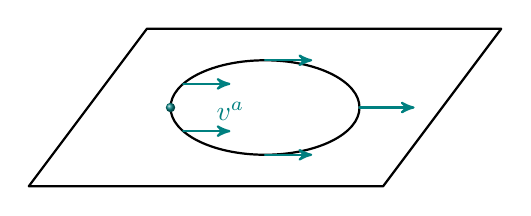
\begin{tikzpicture}
        \draw (0,0) -- (4.5,0) -- (6,2) -- (1.5,2) -- cycle;
        \draw [xshift=3cm,yshift=1cm] (0,0) ellipse (1.2 and .6);
        \draw [xshift=3cm,yshift=1cm,->,teal] (0,.6) -- (.6,.6);
        \draw [xshift=3cm,yshift=1cm,->,teal] (1.2,0) -- (1.9,0);
        \draw [xshift=3cm,yshift=1cm,->,teal] (0,-.6) -- (.6,-.6);
        \draw [xshift=3cm,yshift=1cm,->,teal] ({-1.2*cos(30)},{-.6*sin(30)}) --++ (.6,0) node [above] {$v^a$};
        \draw [xshift=3cm,yshift=1cm,->,teal] ({-1.2*cos(30)},{.6*sin(30)}) --++ (.6,0);
        \shade [xshift=3cm,yshift=1cm,ball color=teal] (-1.2,0) circle (.06);
    \end{tikzpicture}
    \caption{The parallel transport of a vector, $v^a$, around a closed curve in the plane. The vector $v^a$ always ``comes back'' pointing in the same direction as it did initially.}
    \label{3.1}
\end{minipage}
\hfill
\begin{minipage}{.48\textwidth}
    \centering
    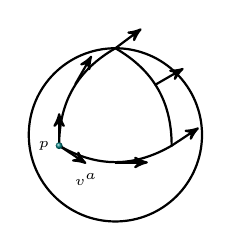
\begin{tikzpicture}[scale=.55]
        \draw (0,0) circle (2);
        \draw (0,2) edge [bend right] ({-3*sqrt(3)/4},-1/4) ({-3*sqrt(3)/4},-1/4) edge [bend right] ({3*sqrt(3)/4},-1/4) ({3*sqrt(3)/4},-1/4) edge [bend right] (0,2) -- cycle;
        \draw [->] (0,2) --++ ({.75*cos(36.8)},{.75*sin(36.8)});
        \draw [->,xshift=9*cos(30)*1pt,yshift=9*sin(30)*1pt] ({3*sqrt(3)/8},1) --++ ({.75*cos(30)},{.75*sin(30)});
        \draw [->] ({3*sqrt(3)/4},-1/4) --++ ({.75*cos(33.4)},{.75*sin(33.4)});
        \draw [->,yshift=(-1/4*1cm-11pt)] (0,0) --++ (.75,0);
        \draw [->] ({-3*sqrt(3)/4},-1/4) --++ ({.75*cos(33.4)},{-.75*sin(33.4)}) node [below] {$\scriptscriptstyle v^a$};
        \draw [->] ({-3*sqrt(3)/4},-1/4) --++ ({.75*cos(90)},{.75*sin(90)}) node [at start,left] {$\scriptscriptstyle p$};
        \draw [->,xshift=-9*cos(30)*1pt,yshift=10*sin(30)*1pt] ({-3*sqrt(3)/8},1) --++ ({.75*cos(60)},{.75*sin(60)});
        \shade [ball color=teal] ({-3*sqrt(3)/4},-1/4) circle (.08);
    \end{tikzpicture}
    \caption{The parallel transport of a vector, $v^a$, around a closed curve on the sphere. In the case shown here of a closed curved composed of three mutually orthogonal segments of great circles, the vector $v^a$ comes back rotated by $90^\circ$.}
    \label{3.2}
\end{minipage}
\end{figure}

Given only the manifold structure of space, we do not have a natural notion of parallel transport. The reason is that the tangent space $V_p$ and $V_q$, of two distinct points $p$ and $q$ are different vector spaces and hence there is no way of saying that a vector at $p$ is the same as a vector at $q$. Thus, the definition of parallel transport requires more than just the manifold structure. It is not difficult to convince oneself that a notion of how to parallel-transport vectors should be equivalent to the knowledge of how to take derivatives of vector fields. If we know how to parallel-transport vectors along a curve, we can define the derivative of a vector field in the direction of the curve; similarly, given a notion of derivative, we can define a vector to be parallel transported if its derivative along the given curve is zero. It turns out to be most convenient to work directly with the notion of a derivative operator, and we shall do so in this chapter. The failure of a vector to return to its original value when parallel transported around an infinitesimal closed curve translates into the lack of commutativity of derivatives. Thus, the notion of curvature can be defined in terms of the failure of successive differentiations on tensor fields to commute. This is the route we shall follow in section 3.2.

From where does this extra structure needed to define parallel transport or a derivative operator arise? We will show in section 3.1 that given a metric (of any signature), there is a unique definition of parallel transport which preserves inner products of all pairs of vectors. Thus, the existence of a metric gives rise to a unique notion of parallel transport and, thus, to an intrinsic notion of the curvature of the manifold. This is the notion of the curvature of a spacetime $(M,g_{ab})$ in which we are interested. However, it is more convenient to proceed by giving a general definition of the notions of derivative operator, parallel transport, and curvature before specializing to the case where they arise from a metric, and we shall proceed in this manner.

Derivative operators and parallel transport are defined in section 3.1, and curvature is defined in section 3.2. In much of our discussion in these sections, we shall follow closely the treatment given in unpublished notes of Geroch. Geodesics are introduced in section 3.3, and the geodesic deviation equation—which characterizes curvature in terms of the failure of initially parallel geodesics to remain parallel—is derived. Finally, section 3.4 discusses methods for computing curvature.

\label{3.2.3}\label{3.2.25}

\section{Derivative Operators and Parallel Transport}
A \emph{derivative operator}, $\nabla$ (sometimes called a \emph{covariant derivative}) on a manifold M is a map which takes each smooth (or merely differentiable) tensor field of type $(k,l)$ to a smooth tensor field of type $(k,l+1)$ and satisfies the five properties listed below. In the index notation, if ${T^{a_1\cdots a_k}}_{b_1\cdots b_l}\in\mathscr{T}(k,l)$, we denote the tensor field resulting from the action of $\nabla$ on $T$ by $\nabla_c{T^{a_1\cdots a_k}}_{b_1\cdots b_l}.$ It is often notationally A
convenient to attach an index directly to the derivative operator and write it as $\nabla_a$, although this is to some extent an abuse of the index notation since $\nabla_a$ is not a dual vector. Expressed in the index notation, the five conditions required of a derivative operator are

\begin{enumerate}
    \item Linearity: For all $A, B\in \mathscr{T} (k,l) $ and $\alpha, \beta\in R$
    \[\nabla_c(\alpha{A^{a_1\cdots a_k}}_{b_1\cdots b_l}+\beta {B^{a_1\cdots a_k}}_{b_1\cdots b_l})=\alpha\nabla_c{A^{a_1\cdots a_k}}_{b_1\cdots b_l}+\beta\nabla_c{B^{a_1\cdots a_k}}_{b_1\cdots b_l}\]
    \item Leibnitz rule: For all $A\in\mathscr{T}(k,l),B\in\mathscr{T}(k',l')$
    \[\nabla_e[{A^{a_l\cdots a_k}}_{b_l\cdots b_l}{B^{c_l\cdots c_k'}}_{d_1\cdots d_l'}]=[\nabla_e{A^{a_l\cdots a_k}}_{b_l\cdots b_l}]{B^{c_l\cdots c_k}}_{d_1\cdots d_l'}+{A^{a_l\cdots a_k}}_{b_1\cdots b_l}[\nabla_e{B^{c_l\cdots c_k'}}_{d_1\cdots d_l'}]\]
    \item Commutativity with contraction: For all $A\in\mathscr{T}(k,l)$
    \[\nabla_{d}({A^{a_1\cdots c\cdots a_k}}_{b_1\cdots c\cdots b_l})={\nabla_{d}A^{a_1\cdots c\cdots a_k}}_{b_1\cdots c\cdots b_l}\]
    \item Consistency with the notion of tangent vectors as directional derivatives on scalar fields: For all $f\in\mathscr{F}$ and all $t^a\in V_p$
    \[t(f)=t^a\nabla_af\]
    \item Torsion free\footnote{If condition 5 is not imposed, it can be shown that there must exist a tensor ${T^c}_{ab}$ antisymmetric in $a$ and $b$ such that $\nabla_a\nabla_bf-\nabla_b\nabla_af=-{T^c}_{ab}\nabla_cf($see problem l). ${T^c}_{ab}$ is called the torsion tensor, and thus our condition 5 states that the torsion tensor vanishes.}: For all $f\in\mathscr{F}$ 
    \[
    \nabla_a\nabla_bf=\nabla_b\nabla_af
    \]
\end{enumerate}

The fifth condition is sometimes dropped, and indeed there are theories of gravitation where it is not imposed. However, in general relativity the derivative operator is assumed to satisfy condition 5 and, unless otherwise stated, all derivative operators considered in this book will be assumed to be torsion free.

It is worth noting that the conditions 4 and 5 together with the Leibnitz rule allow us to derive a simple expression for the commutator of two vector fields $v^a$, $w^b$ in terms of any derivative operator $\nabla_a$. Applied to any smooth function $f$, we have

\begin{equation}
\begin{aligned}\relax
[v,w](f)&=v\{w(f)\}-w\{v(f)\}=v^a\nabla_a(w^b\nabla_bf)-w^a\nabla_a(v^b\nabla_bf)\\
&=\{\upsilon^a\nabla_aw^b-w^a\nabla_av^b\}\nabla_bf
\end{aligned}
\label{3.1.1}
\end{equation}

Thus we have
\begin{equation}
    [v,w]^b=v^a\nabla_aw^b-w^a\nabla_av^b
\end{equation}

Our first important task is to show that derivative operators exist. Let $\psi$ be a coordinate system and let $\{\partial/\partial
x^\mu\}$ and $\{\d x^\mu\} $ be the associated coordinate bases. Then n the region covered by these coordinates we may define a derivative operator, $\partial_a$, called an ordinary derivative, as follows. For any smooth tensor field $T{^{a_1\cdots a_k}}_{b_1\cdots b_k}$ we take its components $T^{\mu_1\cdots\mu_k}$ in this coordinate basis and define $\partial_c{T^{a_1\cdots a_k}}_{b_1\cdots b_l}$ to be the tensor whose components in this coordinate basis are the bartial derivatives $\partial({T^{\mu_1\cdots\mu_k}}_{\nu_1\cdots\nu_l})/\partial x^\sigma$. All five conditions follow immediately from the standard properties of partial derivatives. Indeed, by the equality of mixed partial derivatives, the fifth condition holds for all tensor fields, not just scalar fields. Thus, given a coordinate system $\psi$, we can construct an associated derivative operator $\partial_a.$ Df course, a different choice of coordinate system $\psi'$ will yield a different derivative operator $\partial_a'$, that is, the components of the tensor $\partial_c{T^{a_j\cdots a_k}}_{b_1\cdots b_l}$ in the new (primed) coordinates will $not$ be equal to the partial derivatives of the primed components of ${T^{a_1\cdots a_k}}_{b_1\cdots b_l}$ with respect to the primed coordinates. Thus, a given ordinary derivative operator is coordinate dependent, i.e., it is not naturally associated with the structure of the manifold.

How unique are derivative operators? By condition (4), any two derivative operators $\nabla_a$ and $\tilde{\nabla}_a$ must agree in their action on scalar fields. To investigate their possible disagreements on tensors of the next highest rank, let $\omega_b$ be a dual vector field and consider the difference $\tilde{\nabla}_a(f\omega_b)-\nabla_a(f\omega_b)$ for an arbitrary scalar field $f$. By the Leibnitz rule we have
\begin{equation}
    \tilde{\nabla}_a(f\omega_b)-\nabla_a(f\omega_b)=(\tilde{\nabla}_af)\omega_b+f\tilde{\nabla}_a\omega_b-(\nabla_af)\omega_b-f\nabla_a\omega_b=f(\tilde{\nabla}_a\omega_b-\nabla_a\omega_b)    
    \label{3.1.3}
\end{equation}

where we have used property (4) again. Now at a point $p,\tilde{\nabla}_a\omega_b$ and $\nabla_a\omega_b$ each depend on how $\omega_b$ changes as one moves away from $p$. However, \eqref{3.1.3} shows hat their difference $\tilde{\nabla}_a\omega_b-\nabla_a\omega_b$ depends only on the value of $\omega_b$ at point $p$. To see his, we suppose that $\omega_b'$ equals $\omega_b$ at $p$ and show that we get the same answer if we replace $\omega_b$ by $\omega_b'$. By problem 2 of chapter 2, it follows that since $\omega_b'-\omega_b$ vanishes at $p$ we can find smooth functions, $f_{(a)}$, which vanish at $p$ and smooth dual vector fields, $\mu_b^{(\alpha)}$, such that

\begin{equation}
    \omega_b'-\omega_b=\sum_{\alpha=1}^{n}f_{(\alpha)}\mu_b^{(\alpha)}
    \label{3.1.4}
\end{equation}

Hence, using \eqref{3.1.3}, at point $p$ we have
\begin{equation}
\begin{aligned}
    \tilde{\nabla}_a(\omega_b'-\omega_b)-\nabla_a(\omega_b'-\omega_b)&=\sum_{\alpha}\ab\{\tilde{\nabla}_a\ab(f_{(\alpha)}\mu_b^{(\alpha)})-\nabla_a\ab(f_{(\alpha)}\mu_b^{(\alpha)})\}\\
    &=\sum_{\alpha}f_{(\alpha)}\ab\{\tilde{\nabla}_a\mu_b^{(\alpha)}-\nabla_a\mu_b^{(\alpha)}\}=0
\end{aligned}
\label{3.1.5}
\end{equation}

since each $f_{(\alpha)}=0$ at $p$. Thus, we have
\begin{equation}
    \tilde{\nabla}_a\omega_b'-\nabla_a\omega_b'=\tilde{\nabla}_a\omega_b-\nabla_a\omega_b
    \label{3.1.6}
\end{equation}

which proves our assertion.

Thus, we have shown that $\tilde{\nabla}_a-\nabla_a$ defines a map of dual vectors at $p$ (as opposed to dual vector fields defined in a neighborhood of $p)$ to tensors of type $(0,2)$ at $p$ By property (1), this map is linear. Consequently $(\tilde{\nabla}_a-\nabla_a)$ defines a tensor of type $(1,2)$ at $p$, which we will denote as ${C^c}_{ab}.$ Thus, we have shown that given any two derivative operators $\tilde{\nabla}_a$ and $\nabla_a$ there exists a tensor field ${C^c}_{ab}$ such that
\begin{equation}
    \nabla_a\omega_{b}=\tilde{\nabla}_a\omega_{b}-{C^c}_{ab}\omega_c
    \label{3.1.7}
\end{equation}

This displays the possible disagreements of the actions of $\nabla_a$ and $\tilde{\nabla}_a$ on dual vecton fields.

A symmetry property of ${C^c}_{ab}$ follows immediately from condition (5). If we let $\omega_{b}=\nabla_{b}f=\tilde{\nabla}_{b}f$, we find
\begin{equation}
    \nabla_a\nabla_{b}f=\tilde{\nabla}_a\tilde{\nabla}_{b}f-{C^c}_{ab}\nabla_cf
    \label{3.1.8}
\end{equation}

Since both $\nabla_a\nabla_bf$ and $\tilde{\nabla}_a\tilde{\nabla}_bf$ are symmetric in $a$ and $b$, it follows that ${C^c}_{ab}$ must also have this property
\begin{equation}
    {C^c}_{ab}={C^c}_{ba}
    \label{3.1.9}
\end{equation}

\eqref{3.1.9}, of course, need not hold if the torsion-free requirement is dropped.

The difference in the action of $\tilde{\nabla}_a$ and $\nabla_a$ on vector fields and all higher rank tenson fields is determined by \eqref{3.1.7}, the Leibnitz rule, and property (4). For every vector field $t^a$ and one-form field $\omega_a$, property (4) tells us that
\begin{equation}
    (\tilde{\nabla}_a-\nabla_a)(\omega_bt^b)=0
    \label{3.1.10}
\end{equation}

On the other hand, by the Leibnitz rule, we have
\begin{equation}
    (\tilde{\nabla}_a-\nabla_a)(\omega_bt^b)=({C^c}_{ab}\omega_c)t^b+\omega_b(\tilde{\nabla}_a-\nabla_a)t^b
    \label{3.1.11}
\end{equation}

Thus, index substituting on contracted indices, we find
\begin{equation}
    \omega_{b}\ab[(\tilde{\nabla}_a-\nabla_a)t^{b}+{C^{b}}_{ac}t^c]=0
    \label{3.1.12}
\end{equation}

for all $\omega_b$. This implies
\begin{equation}
    \nabla_at^{b}=\tilde{\nabla}_at^b+{C^{b}}_{ac}t^c
    \label{3.1.13}
\end{equation}

Continuing in a similar manner, we can derive the general formula for the action of $\nabla_a$ on an arbitrary tensor field in terms of $\tilde{\nabla} _a$ and $\tilde{c} _{ab}^c$. For $T\in\mathscr{T}(k,l)$ we find
\begin{equation}
    \nabla_a{T^{b_1\cdots b_k}}_{c_1\cdots c_l}=\tilde{\nabla}_a{T^{b_1\cdots b_k}}_{c_1\cdots c_l}+\sum_iC^{b_1}{}_{ad}T^{b_1\cdots d\cdots b_k}{}_{c_1\cdots c_l}-\sum_jC^d{}_{ac_j}T^{b_1\cdots b_l}{}_{c_1\cdots d\cdots c_l}
    \label{3.1.14}
\end{equation}

Thus, the difference between the two derivative operators $\nabla_a$ and $\tilde{\nabla}_a$ is completely characterized by the tensor field ${C^c}_{ab}.$ Conversely, it is not difficult to check that if $\tilde{\nabla}_a$ is a derivative operator and ${C^c}_{ab}$ is an arbitrary smooth tensor field which is symmetric in its lower indices, then $\nabla_{a}$ defined by equation (3.1.14) will also be a derivative operator. This shows that there is a great deal of freedom involved in the choice of a derivative operator, as on an $n$-dimensional manifold ${C^c}_{ab}$ has $n^2(n+1)/2$ independent components to be specified at each point.

The most important application of equation (3.Î.14) arises from the case where $\tilde{\nabla}_{a}$
is an ordinary derivative operator $\partial_{a}$. In this case, the tensor field ${C^c}_{ab}$ is denoted $\Gamma_{ab}^{c}$ and called a $Christoffel$ symbol. Thus, for example, we write

$$
\nabla_{a}t^{b}\:=\:\partial_{a}t^{b}\:+\:\Gamma_{\:ac}^{b}t^{c}
$$
(3.1.15) Since we know how to compute the ordinary derivative associated with a given coordinate system, equation $(\dot{3}.1.15)$ (and, more generally, eq.[3.1.14]with $\partial_{a}$ and $\Gamma_{ac}^b$ replacing $\tilde{\nabla}_a$ and $\bar{C}_{ac}^b)$ tells us how to compute the derivative $\nabla_a$ if we know $\Gamma_{ac}^b$ Note that, as defined here, a Christoffel symbol is a tensor field associated with the derivative operator $\nabla_a$ and the coordinate system used to define $\partial_a$. However, if we change coordinates, we also change our ordinary derivative operator from $\partial_a^{\prime}$ to $\partial_a^{\prime}$ and thus we change our tensor $\Gamma_{ab}^\mathrm{\vdots c}$ to a new tensor $\Gamma_{ab}^{\prime c}$. Hence the coordinate components of $\Gamma_{ab}^c$ in the unprimed coordinates will not be related to the components of $\Gamma_{ab}^{\ddots}$ in the primed coordinates by the tensor transformation law, equation (2.3.8), since we change tensors as well as coordinates.

Given a derivative operator $\nabla_{a}$ we can define the notion of the parallel transport of a vector along a curve $C$ with a tangent $t^a$. A vector $v^a$ given at each point on the curve is said to be parallelly transported as one moves along the curve if the equation
(3.1.16) $t^{a}\nabla_{a}v^{b}=0$
is satisfied along the curve. More generally, one can define the parallel transport of a tensor of arbitrary rank by

(3.1.17) 
$$
t^{a}\nabla_{a}T^{b_{1}\cdots b_{k}}_{c_{1}\cdots c_{l}}=0\quad.
$$

Choosing a coordinate system and using equation (3.1.15), we can express equation (3.1.16) as

(3.1.18) 
$$
t^{a}\partial_{a}v^{b}+t^{a}{\Gamma^{b}}_{ac}v^{c}=0\quad,
$$

or, in terms of components in the coordinate basis and the parameter $t$ along the curve,

(3.1.19) 
This shows that the parallel transport of $\upsilon^{a}$ depends only on the values of $v^a$ on the curve, so we may consider the parallel transport properties of vectors defined only along the curve as opposed to vector fields. Furthermore, from the properties of ordinary differential equations it follows that equation (3.1.19) always has a unique solution for any given initial value of $v^a$. Thus, a vector at a point $p$ on the curve uniquely defines a “parallel transported vector" everywhere else on the curve. We may use this notion of parallel transport to identify (i.e., map into each other) the tangent spaces $V_p$ and $V_q$ of points $p$ and $q$ if we are given a derivative operator and a curve connecting $p$ and $q$. The mathematical structure arising from such a curve-

\section{Curvature}
% \begin{equation}
% \nabla_a\nabla_b\omega_c-\nabla_b\nabla_a\omega_c=R_{abc}^d\omega_d
%     \label{3.2.3}
% \end{equation}

% \begin{equation}
% R_{ac}=R_{abc}^b
%     \label{3.2.25}
% \end{equation}

\section{Geodesics}
\section{Methods for Computing Curvature}

% \includepdf[pages=17-30]{document}
\chapter{Einstein's Euqation}

% \section{The Geometry of Space in Prerelativity Physics; General and Special Covariance}
% \section{Special Relativity}
\label{4.2.2}
% \begin{equation}
%     \eta_{ab}=\sum_{\mu,\nu=0}^3\eta_{\mu\nu}(\d x^\mu)_a(\d x^\nu)_b
%     \label{4.2.2}
% \end{equation}

% \section{General Relativity}
% \section{Linearized Gravity: The Newtonian Limit and Gravitational Radiation}

% \includepdf[pages=31-42]{document}
\chapter{Homogeneous, Isotropic Cosmology}
% \section{Homogeneity and Isotropy}
% \section{Dynamics of a Homogeneous, Isotropic Universe}
% \section{The Cosmological Redshift; Horizons}
% \section{The Evolution of Our Universe}

% \includepdf[pages=43-51]{document}
\chapter{The Schwarzschild Solution}
As described in the previous chapter, the theory of general relativity has made a number of strikingly successful predictions concerning the spacetime structure of our universe. However, cosmological observations presently are not good enough to provide stringent quantitative tests of general relativity. Such quantitative tests are provided by the gravitational fields occurring in our solar system, where precise measurements can be made. Thus, it is of great interest to determine the solution of Einstein's equation corresponding to the exterior gravitational feld of a static, spherically symmetric body (such as are our Sun and many other bodies, to an excellent approximation). This problem was solved by Karl Schwarzschild (1916a), only a few months after Einstein published his vacuum field equations. The Schwarzschild solution without question remains one of the most important known exact solutions of Einstein's equation.

As was previously discussed in section 4.4a, in the slow motion, weak field limit, the predicitons of general relativity reduce to those of Newtonian theory. However, the Schwarzschild solution, which describes the exact exterior field of a spherical body, predicts tiny departures from Newtonian theory for the motion of planets in our solar system, and, in addition, predicts the ``bending of light'', the gravitational redshift of light, and ``time delay'' effects. These four predictions have been accurately confirmed by precise measurements. Indeed, except for the binary pulsan measurements (see the end of chapter 4), the predictions of the Schwarzschild solution in the weak field regime of our solar system are the only predictions of general relativity to have been tested in a quantitatively precise manner.

But the Schwarzschild solution has provided us with a great deal more than the ability to predict tiny effects occurring in our solar system. As will be discussed further in section 6.2, sufficientlymassivebodiesareunabletosupportthemselves against complete gravitational collapse. After the collapse of a spherical body has occurred, the entire spacetime geometry will be described by the Schwarzschild solution, and thus the Schwarzschild solution tells us a great deal about the strong field behavior of general relativity. As will be seen in section 6.4, the vacuum Schwarzschild solution describing the end-product of gravitational collapse contains a spacetime singularity which is hidden within a black hole.

We shall derive the Schwarzschild solution in section 6.1, using the tetrad method of section 3.4b. In section 6.2 we consider the interior matter sources of the exterion vacuum Schwarzschild solution and thereby derive the relativistic equations of stellar structure. The timelike and null geodesics of the Schwarzschild metric are studied in section 6.3 and are used there to make predictions for the four tests of general relativity: the gravitational redshift, the precession of Mercury's orbit, the bending of light, and the ``time delay'' of light. Finally, in section 6.4 we examine the strong field regime of the vacuum Schwarzschild solution.

% \section{Derivation of the Schwarzschild Solution}
% \section{Interior Solutions}
% \section{Geodesics of Schwarzschild: Gravitational Redshift, Perihelion Precession, Bending of Light, and Time Delay}
% \section{The Kruskal Extension}

% \includepdf[pages=53-59]{document}
\end{document}